\documentclass[11pt]{article}
\usepackage{times}
\usepackage{amsmath,amsthm,amssymb,setspace,enumitem,epsfig,titlesec,verbatim,color,array,eurosym,multirow}
\usepackage[sort&compress]{natbib}
\usepackage[footnotesize,bf]{caption}
\usepackage[margin=2.5cm, includefoot, footskip=30pt]{geometry}
\usepackage{standalone}
\usepackage{tikz}
\usepackage{subcaption}
\usepackage{hyperref}
\usepackage{tabularx}
\usepackage{booktabs}
\usepackage[ruled,vlined]{algorithm2e}
\smallskip % Erlaubt kleine Abstaende zwischen Paragraphen, falls es dem Seitenlayout hilft
\renewcommand{\baselinestretch}{1.3}
\newcommand{\R}{\mathbb{R}}

\definecolor{darkblue}{rgb}{0,0,.8}
\definecolor{darkgreen}{rgb}{0,0.5,0.1}
\newcommand{\matlabfunc}[1]{\textcolor{darkblue}{#1}}
\newcommand{\matlabcomment}[1]{\textcolor{darkgreen}{#1}}
\newcommand{\christian}[1]{\textcolor{blue}{\textbf{CH}: #1}}
\newcommand{\alex}[1]{\textcolor{red}{\textbf{AL}: #1}}

%% Adding shortcut commands to refer to our figures %%
\newcommand{\FigEvoProc}{{\bf Fig.~1}}
\newcommand{\FigInvAnalysis}{{\bf Fig.~2}}
\newcommand{\FigResultsOverPara}{{\bf Fig.~3}}


\titleformat{\section}{\sffamily \fontsize{12}{14}\bfseries}{\thesection}{1em}{}
\titleformat{\subsection}{\sffamily \fontsize{11.5}{11.5}\bfseries}{\thesubsection}{1em}{}

\usepackage{tikz}
\usetikzlibrary{arrows}

\tikzset{
  treenode/.style = {align=center, inner sep=0pt, text centered,
    font=\sffamily},
  arn_n/.style = {treenode, circle, white, font=\sffamily\bfseries, draw=black, inner sep=-6pt,
    fill=black, text width=1.5em},% arbre rouge noir, noeud noir
  arn_r/.style = {treenode, circle, red, 
    text width=1.5em, very thick, inner sep=4pt},% arbre rouge noir, noeud rouge
  arn_x/.style = {treenode, rectangle, draw=black,
    minimum width=0.5em, minimum height=0.5em}% arbre rouge noir, nil
}

\newtheoremstyle{plainCl1}% name
{9pt}%      Space above, empty = 'usual value'
{9pt}%      Space below
{\it}% 	   Body font
{}%         Indent amount (empty = no indent, \parindent = para indent)
{\bfseries}% Thm head font
{.}%        Punctuation after thm head
{0.2cm}% Space after thm head: \newline = linebreak
{}%         Thm head spec

\newtheoremstyle{plainCl2}% name
{9pt}%      Space above, empty = 'usual value'
{9pt}%      Space below
{\it}% 	   Body font
{}%         Indent amount (empty = no indent, \parindent = para indent)
{\bfseries}% Thm head font
{$'$.}%        Punctuation after thm head
{0.2cm}% Space after thm head: \newline = linebreak
{}%         Thm head spec

\newcommand{\splitatcommas}[1]{%
  \begingroup
  \begingroup\lccode`~=`, \lowercase{\endgroup
    \edef~{\mathchar\the\mathcode`, \penalty0 \noexpand\hspace{0pt plus 1em}}%
  }\mathcode`,="8000 #1%
  \endgroup
}

\theoremstyle{plainCl1}
\newtheorem{Claim}{Claim}
\newtheorem{Thm}{Theorem}
\newtheorem{Prop}{Proposition}
\newtheorem*{Lem}{Lemma}
\newtheorem{Cor}{Corollary}
\newtheorem*{Def}{Definition}

\theoremstyle{plainCl2}
\newtheorem{Claim2}{Claim}

\title{
\bf  \sffamily \LARGE Evolution of cooperation among individuals with limited payoff memory\\}
\date{}
\author{Christian Hilbe, Nikoleta E. Glynatsi, Alex McAvoy}

\begin{document}
\maketitle

\begin{abstract}

\end{abstract}

\section{Introduction}

One of the most important applications of evolutionary game theory is the
evolution of cooperation. Why is it that some individuals choose to help others,
increasing their payoff, at the expense of decreasing one’s own? In evolutionary
game theory, individuals are not required to be rational, instead they adapt
strategies based on mutation and exploration. Strategies are more likely to
spread if they have a high fitness either because the individuals who adopt them
have more offspring, or because they are imitated more often. The fitness of a
strategy is not constant but depends on the composition of the population.
Individuals interact based on their strategies with other members of the
population and the payoffs they yield are translated into fitness.

It is commonly assumed that fitness is equivalent to the mean distribution of
types in the population. These payoffs assume that individuals can interact with
the entire population several times and remember each and every outcome. Thus,
they imply that individuals have a perfect memory. However, when they make
decisions in each turn they are assumed to have very limited memory. To be
precise, most of the works in the literature focus on naive subjects who can
only choose from a restricted set of strategies~\cite{Nowak1992tit}, or who do
not remember anything beyond the outcome of the very last round~\cite{Baek2016}.
Note that there are a few notable exceptions~\cite{Hauert1997, Stewart2016}.

The perfect memory assumption is not only unrealistic but it also creates this
curious inconsistency. This has led us to question how robust is our
understanding of cooperation. In this work, we explore whether direct
reciprocity can evolve if individuals only remember a minimum of social
information. Though we are not the first to question the assumptions of
estimating fitness~\cite{Roca2006}, we are the first to explore the effect of
payoff memory.

Initially, we consider two extreme scenarios. The first is the classical
scenario of the expected payoffs and the alternative scenario where individuals
update their strategies only based on the very last payoff they obtained. In the
later sections, we allow individuals more memory. More specifically, they can
remember up to two turns and up to two interactions. We present results on
several social dilemmas which include the prisoner’s dilemma and the donation
game, the snowdrift game, the stag hunt game and the harmony game.

The remainder of the paper is organized as follows. Section~\ref{section:model}
describes the model. Section~\ref{section:results} presents the results of the
simulations. Finally, section~\ref{section:conclusions} outlines the main
conclusions.

% Early results for the repeated prisoner’s dilemma and for the snowdrift game
% suggest that memory size can have a considerable effect on the evolutionary
% dynamics. As a rule of thumb, we observe that individuals with limited memory
% tend to adopt less generous strategies and they achieve less cooperation than in
% the classical scenario. In contrast, in the stag-hunt and the harmony game, the
% impact of memory is less striking. Here individuals with limited memory perform
% nearly as well as individuals with full memory.

\section{Model Setup}\label{section:model}

We consider a population of \(N\) players (\(N\) is even) where mutations are
sufficiently rare. Thus, at any point in time there are at most two
different strategies present in the population; a \textit{resident} strategy
and a \textit{mutant} strategy. We assume a pairwise process where
strategies spread because they are imitated more often.

Each step of the evolutionary process consists of two stages, a game stage and
an updating stage. In the game stage each individual is randomly matched with
some other individual in the population to interact for a number of turns, where
subsequent turns occur with a fixed probability $\delta$. At each turn they
can choose to either cooperate (\(C\)) or to defect (\(D\)), and thus, at
each turn the possible outcomes are \(CC, CD, DC\) and \(DD\). The payoffs
depend on the outcome. If both cooperate they receive the reward payoff
\(R\), whereas if both defect they receive the punishment payoff \(P\).
If one cooperates but the other defects, the defector receives the temptation to
defect, \(T\), whereas the cooperator receives the sucker's payoff, \(S\).
We denote the payoffs of an individual as \(\mathcal{U} = (R, S, T, P)\).

We assume herein that individuals use \textit{reactive strategies} to make
decisions in each turn. Reactive strategies are a set of memory-one strategies
that only take into account the previous action of the opponent. They can be
written explicitly as a vector \(\in \R_{3}\), more specifically, a reactive
strategy \(s\) is given by \(s=(y, p, q)\) where \(y\) is the probability that
the strategy opens with a cooperation and \(p, q\) are the probabilities that
the strategy cooperates given that the opponent cooperated and defected
equivalently.

In the updating stage, two players are randomly drawn from the population, a
`learner' and a `role model'. Given that the learner's payoff $u_L\!\in\!
\mathcal{U}$ and that the role model's payoff $u_{RL}\!\in\! \mathcal{U}$, we
assume the learner adopts the role model's strategy based on the Fermi
distribution function,

\begin{equation} \label{Eq:rho}
  \rho(u_{L}, u_{RM}) = \frac{1}{1\!+\! \exp^{\!-\!\beta (u_{RM}\!-\!u_{L})}}.
\end{equation}

where $\beta\!\ge\!0$ is the relative influence of the payoffs on adopting the 
strategy of the other. We refer to $\beta$ as the intensity of selection.

This basic evolutionary step is repeated until either the mutant strategy goes
extinct, or until it fixes in the population. If the mutant fixes in the
population then the mutant strategy becomes the new resident strategy. After
either outcome we introduce a new mutant strategy uniformly chosen from all
reactive strategies at random, and we set the number of mutants to $1$. This
process of mutation and fixation/extinction is then iterated many times.

The perfect memory assumption occurs at the updating stage. The learner and the
role model are assumed to interact with a representative sample of the
population, and they remember all interactions they participate in. Thus, their
updating payoffs are based on the mean payoff they achieved over all the
interactions. These payoffs are referred to as the expected payoffs. We will
compare the expected payoffs to payoffs that are calculated when the role model
and learner do not remember all of their interactions. In order to account for
the effect of these different methods, we explore the cooperation rate within
the resident population over multiple generations. More details on our
methodology are found in Appendix~\ref{appendix:methods}.


\section{Results}\label{section:results}
\subsection{Updating payoffs based on the last round with another member of the population}\label{section:donation}

In this section we explore the case where the updating payoffs are based on the
last round payoff achieved against another member of the population. We compare
this to the expected payoffs. We assume that individuals interact in a donation
game  where each can cooperate by providing a benefit \(b\) to the other
player at their cost \(c\), with \(0 < c < b\). Thus, \(T=b, R=b-c, S=-c, P=0\).

Figure~\ref{fig:expected_and_stochastic_for_donation} shows simulations results
for the described process of section~\ref{section:model}.
Figure~\ref{fig:expected_and_stochastic_for_donation}~depicts the evolving
conditional cooperation probabilities $p$ and $q$. The discount factor~$\delta$
is comparably high, thus the opening move \(y\) is a transient
effect and has no effect on the outcome. The left panel corresponds to the
standard scenario considered in the literature. It considers players who use
expected payoffs to update their strategies. The right panel shows the scenario
considered herein, in which players update their strategies based on their last
round’s payoff. The top panels assume a benefit \(b\) of 3, whereas the bottom
assume a benefit of 10.

The figure suggests that when updating is based on expected payoffs, players
tend to be more generous and more cooperative. The $q$-values are higher on
average which suggests that individuals tend to be more generous when it comes
to cooperating after being at the receiving end of a defection. %This is a known result no? Nowak 1992
The average cooperation rate within the resident population is strictly higher
when expected payoffs are considered. The difference between the two methods for
both the values of \(b\) are statistically significant. This contrast becomes
more obvious for \(b=10\). More specifically the average cooperation drops from
97\% to 51\%. The residents of the population cooperated on average 97\% of the
times in one case and only 57\% in the other.

\begin{figure}[!htbp]
    \centering
    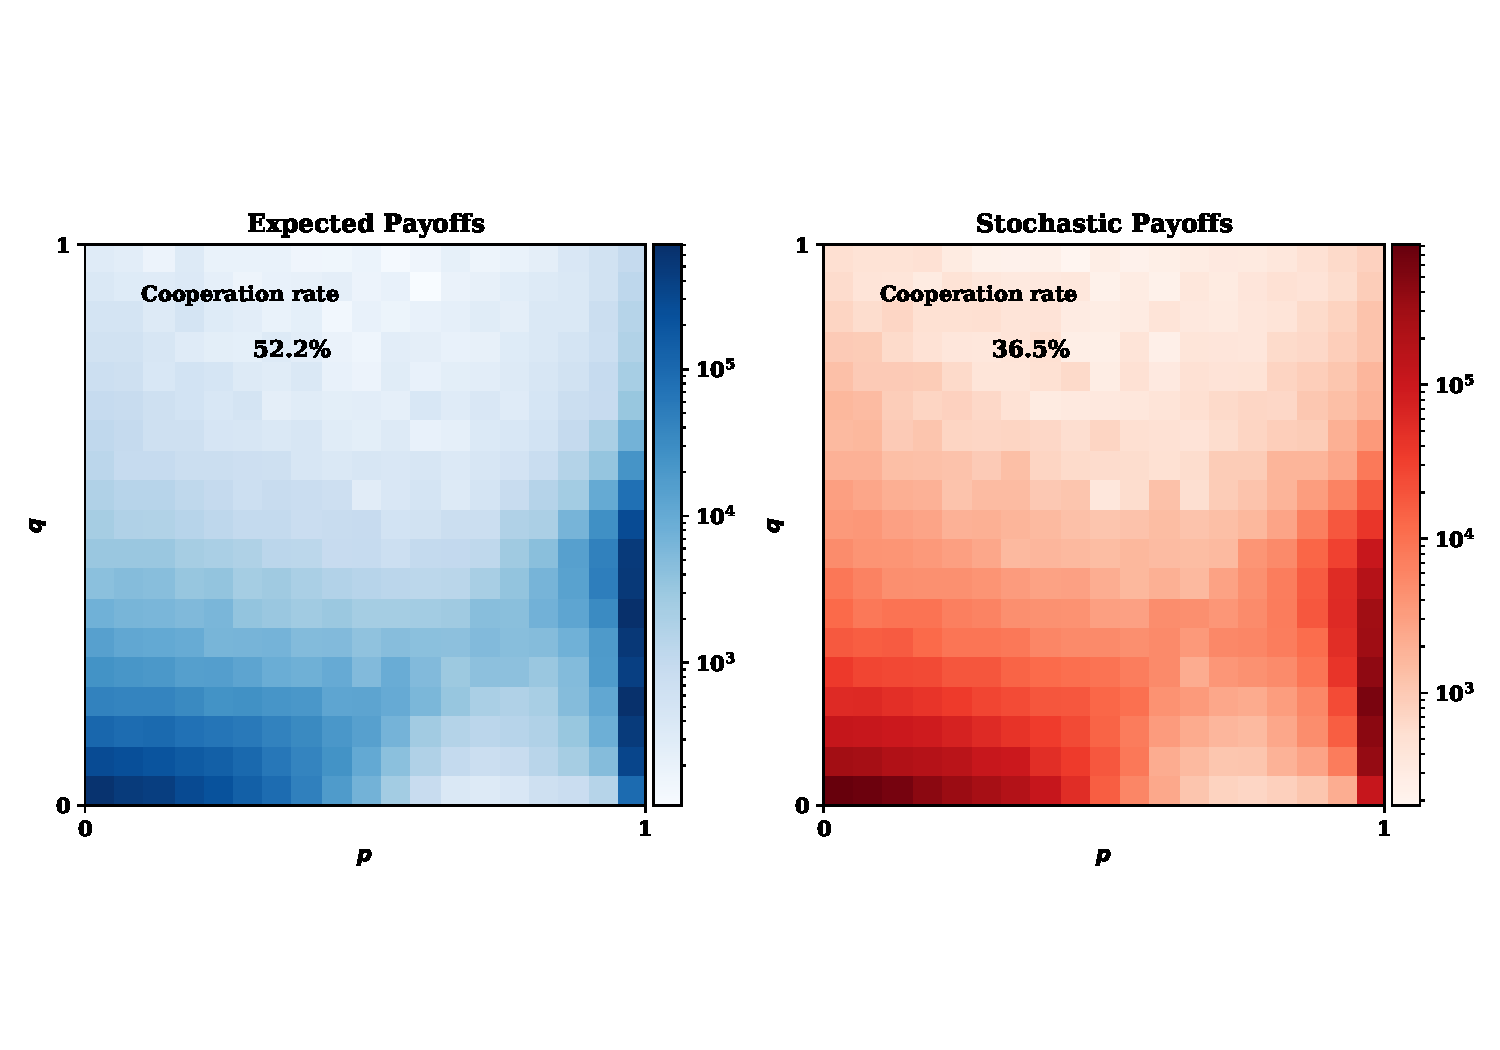
\includegraphics[width=.75\textwidth]{static/expected_and_stochastic_for_donation_game.pdf}\vspace{-3cm}
    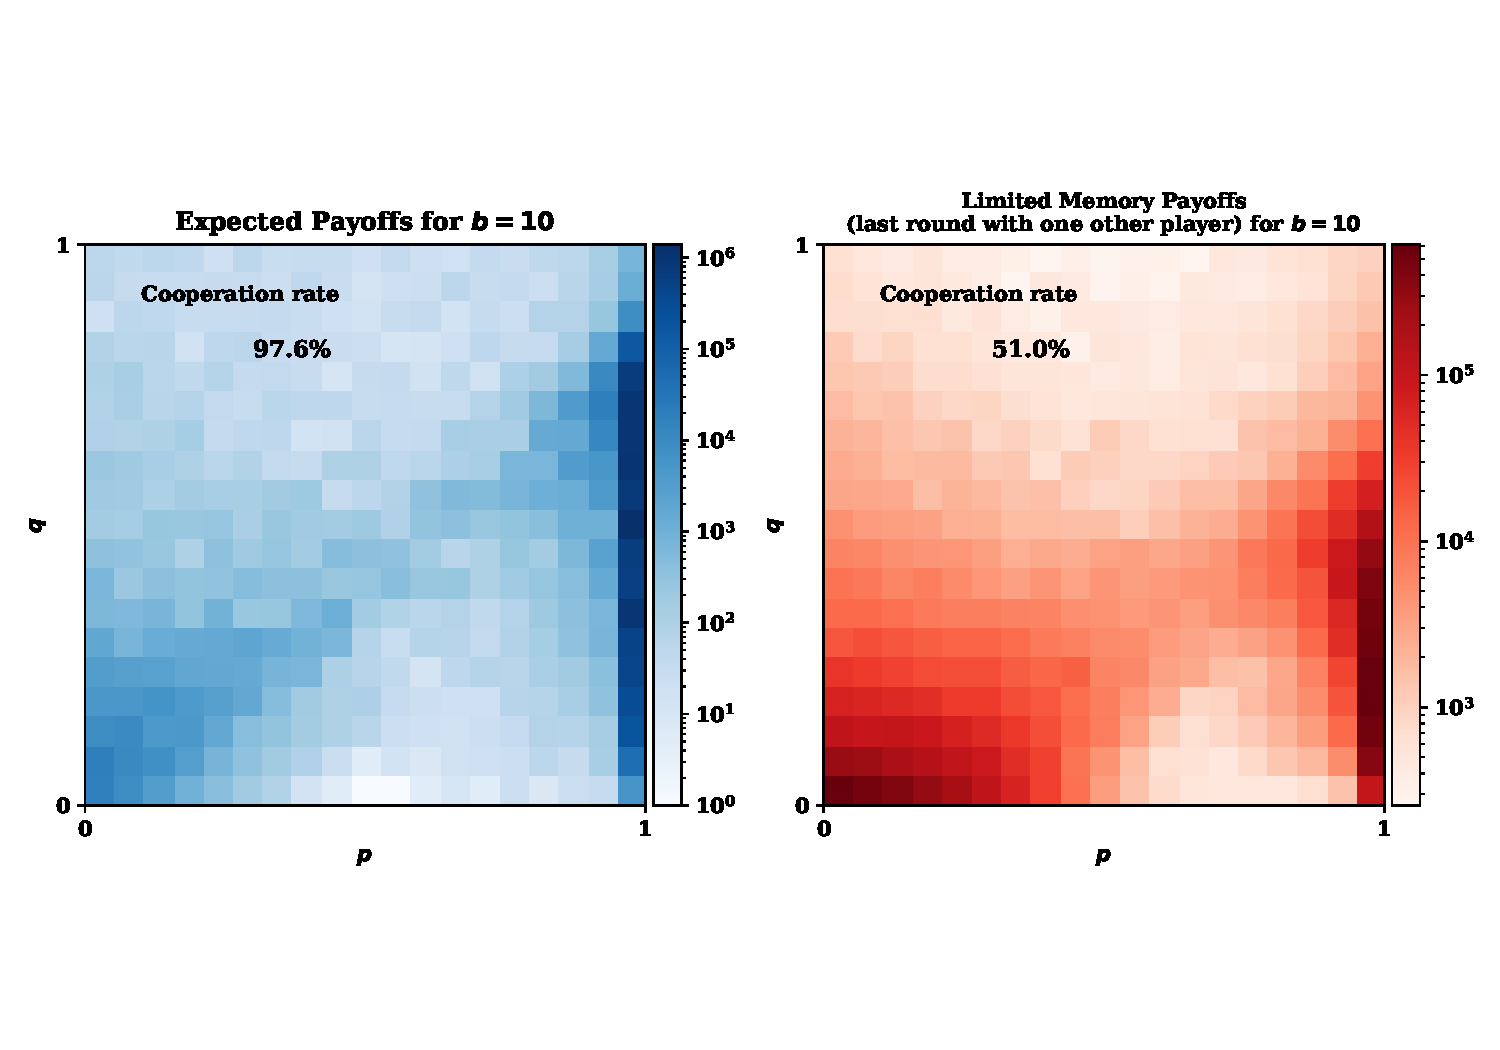
\includegraphics[width=.75\textwidth]{static/expected_and_stochastic_for_donation_game_b_10.pdf}
    \caption{{\bf Evolutionary dynamics under expected payoffs and last round with one interaction payoffs.} 
    We have run two simulations of the evolutionary process described in
    section~\ref{section:model} for $T\!=\!10^7$ time steps. For each time step,
    we have recorded the current resident population ($y,p,q$). Since simulations
    are run for a relatively high continuation probability of $\delta\!=\!0.999$, we
    do not report the players' initial cooperation probability $y$. The graphs show
    how often the resident population chooses each combination ($p,q$) of
    conditional cooperation probabilities in the subsequent rounds. ({\bf A}) If
    players update based on their expected payoffs, the resident population
    typically applies a strategy for which $p\!\approx\!1$ and
    $q\!\le\!1\!-\!c/b\!=\!0.9$. ({\bf B})
    When players update their strategies based on their realized payoffs in the last
    round, there are two different predominant behaviors. The resident population
    either consists of defectors (with $p\!\approx\!q\!\approx\!0$) or of
    conditional cooperators. In the latter case, the maximum level of $q$ consistent
    with stable cooperation is somewhat smaller compared to the expected-payoff
    setting, $q\!<\!0.5$. The cooperation rate within the resident population
    (averaged over all games and over all time steps) is close to 100\%. Parameters:
    $N\!=\!100$, $c\!=\!1$, $\beta\!=\!1$, $\delta\!=\!0.999$.}
    \label{fig:expected_and_stochastic_for_donation}
\end{figure}

We further explore the effect of the benefit,
Figure~\ref{fig:cooperation_rate_over_benefit}. The figure suggests that the
expected payoffs always overestimate cooperation. For the limited memory
payoffs, the cooperation rate remains unchanged at approximately 50\% once \(b =
5\). The highest cooperation rate that was achieved was 0.51 when  the last
round payoff is considered. In comparison, when the expected payoffs were used
the highest average cooperation rate was 0.97.

\begin{figure}[!htbp]
  \centering
  \begin{subfigure}{.5\textwidth}
    \centering
    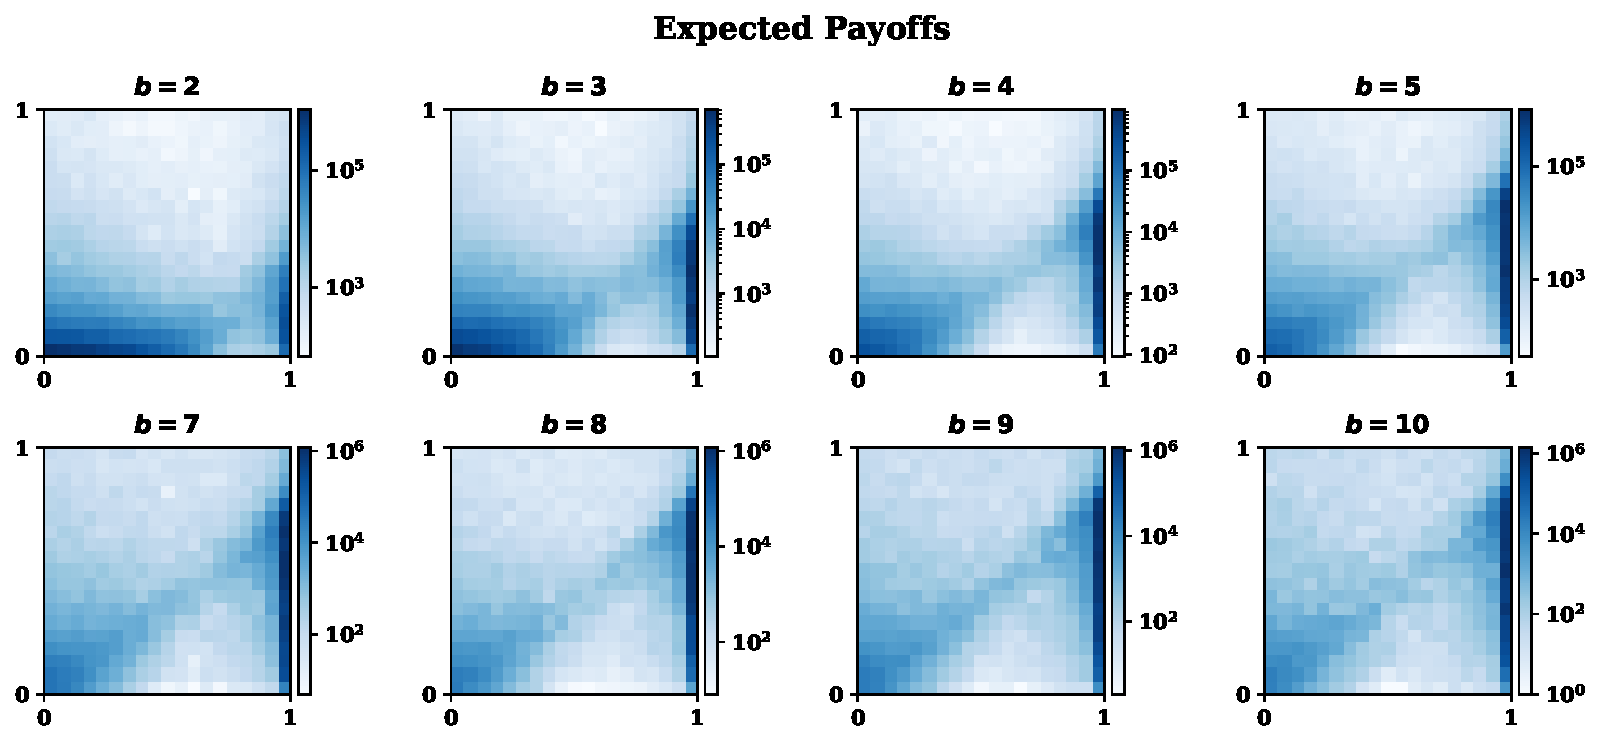
\includegraphics[width=\textwidth]{static/expected_for_beta.pdf}
    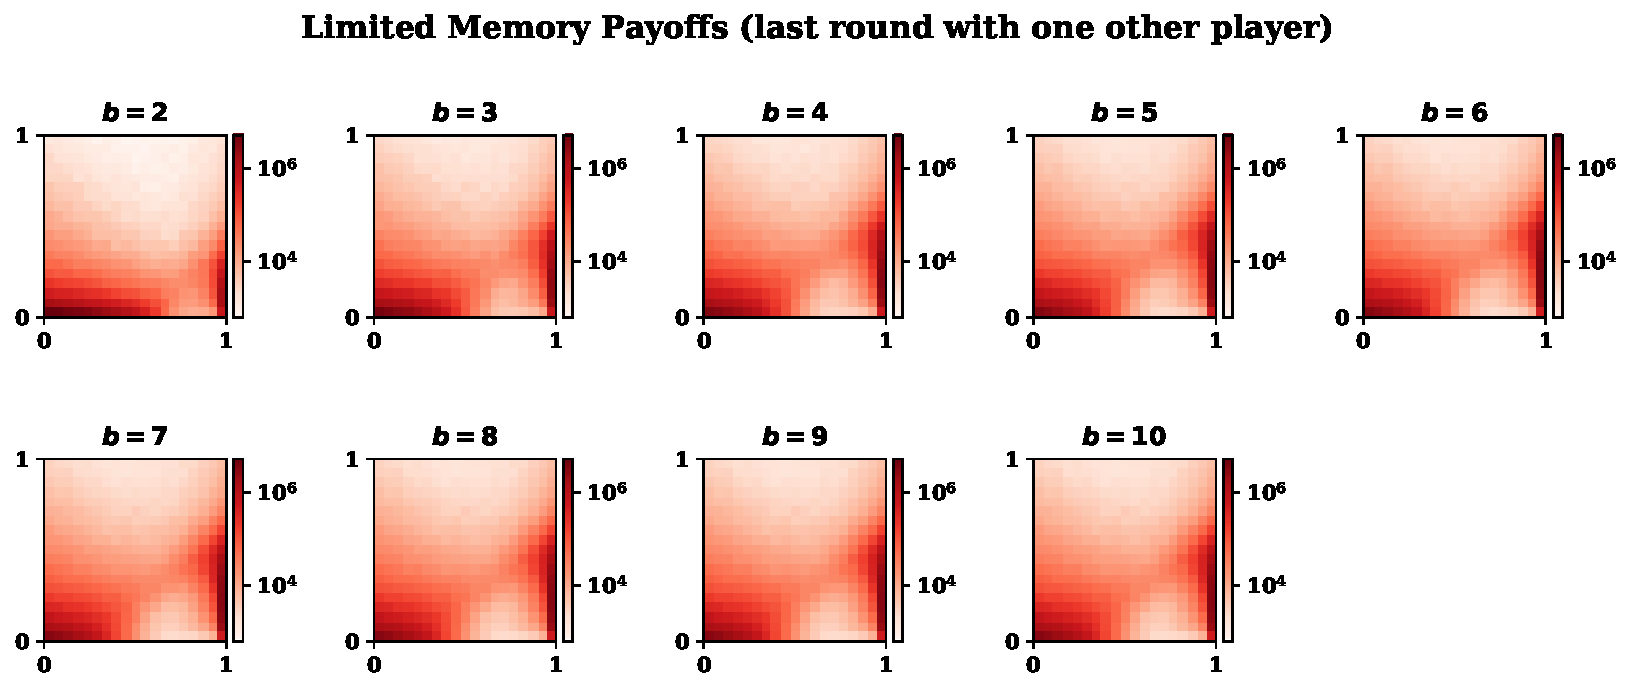
\includegraphics[width=\textwidth]{static/stochastic_for_beta.pdf}
  \end{subfigure}%
  \begin{subfigure}{.5\textwidth}
    \centering
    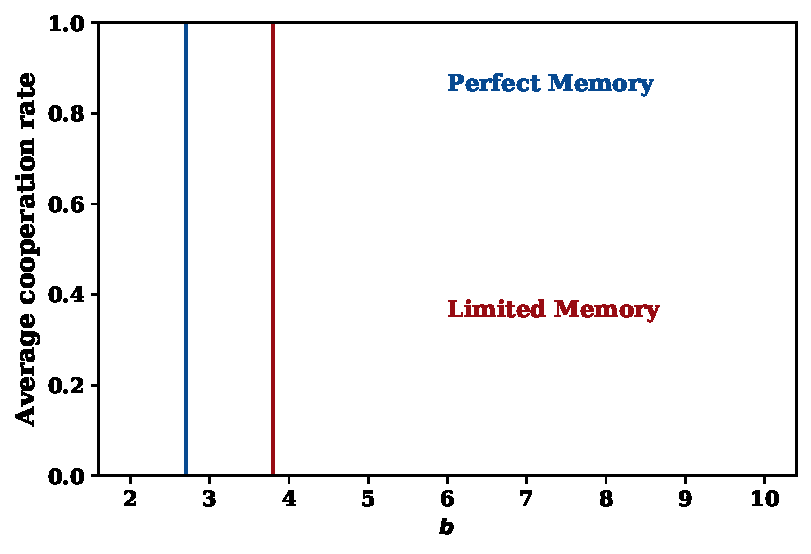
\includegraphics[width=\textwidth]{static/cooperation_rate_over_b.pdf}
  \end{subfigure}
  \caption{{\bf The evolution of cooperation for different benefit values.} 
  We vary the benefit of defection $b$. In all cases, expected payoffs appear to
  overestimate the average cooperation rate the population achieves. ({\bf A})
  the probabilities \(p, q\) for resident population over \(10^7\) time steps
  for each benefit value. ({\bf B}) The cooperation rate within the resident population
  (averaged over all games and over all time steps) over the benefit.
  Unless
  explicitly varied, the parameters of the simulation are $N\!=\!100$,
  $c\!=\!1$, $\beta\!=\!1$, $\delta\!=\!0.99$. Simulations are run
  for $T\!=\!5\times 10^6$ time steps for each parameter
  combination.}\label{fig:cooperation_rate_over_benefit}
\end{figure}

Figure~\ref{fig:cooperation_rate_over_betas} illustrates results for various
runs of the evolutionary process where we vary the strength of selection. For
weak selection, \(\beta < 1\), the updating payoffs have no effect. The evolved
population and the average cooperating rate are the same for both approaches.
However for strong selection, it can be seen that the cooperating rate increases
with \(beta\), when expected payoffs are used. However, when limited memory
payoffs are used the cooperating rate decreases.

\begin{figure}[!htbp]
  \centering
  \begin{subfigure}{.65\textwidth}
    \centering
    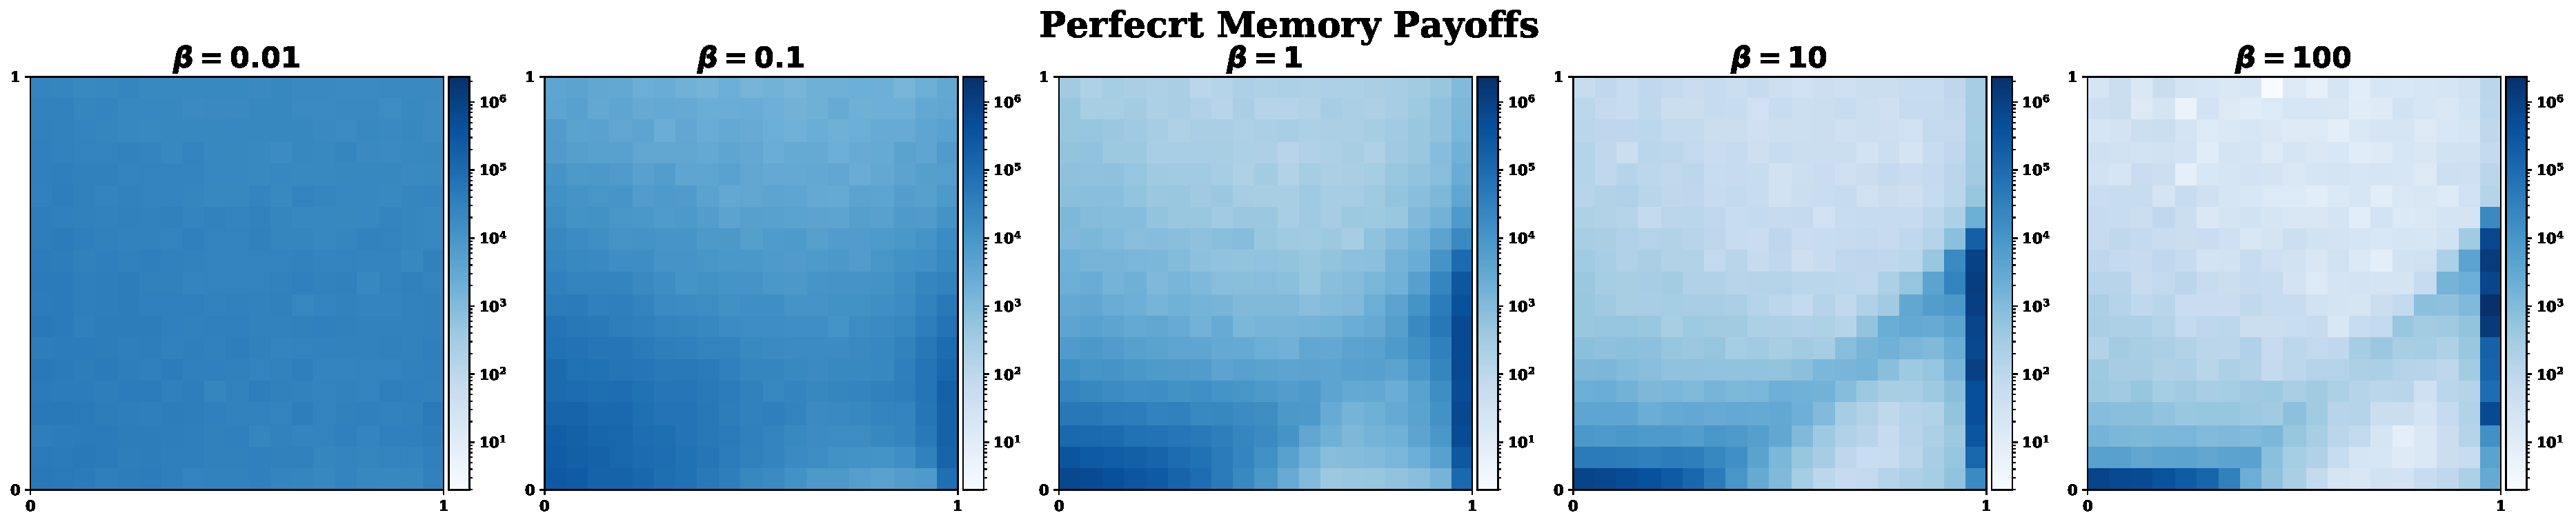
\includegraphics[width=\textwidth]{static/expected_for_selection_strenght.pdf}
    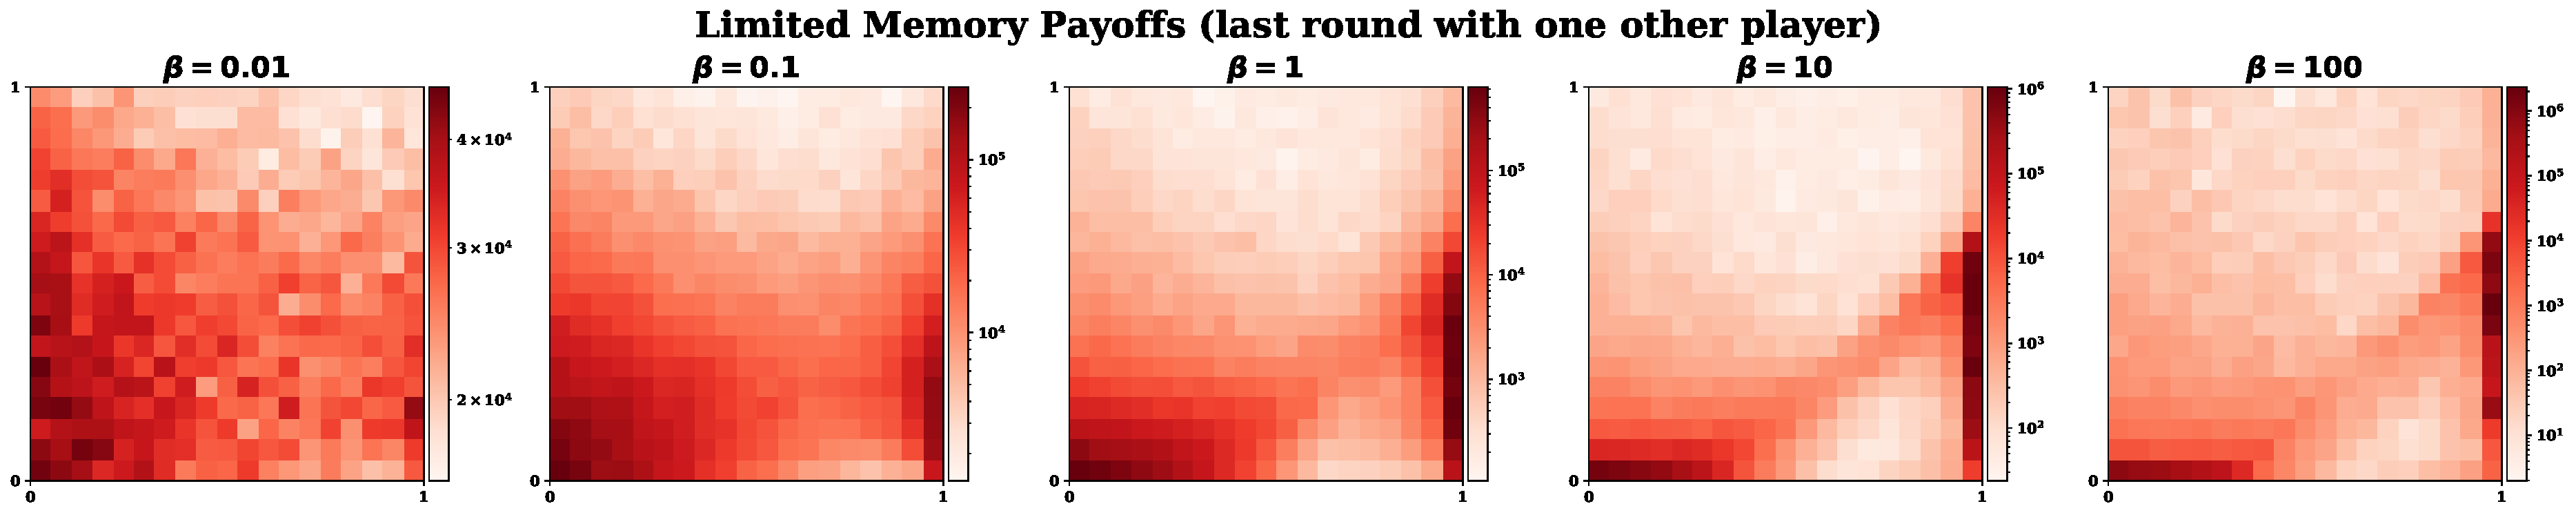
\includegraphics[width=\textwidth]{static/stochastic_for_selection_strenght.pdf}
  \end{subfigure}%
  \begin{subfigure}{.35\textwidth}
    \vspace{.3cm}
    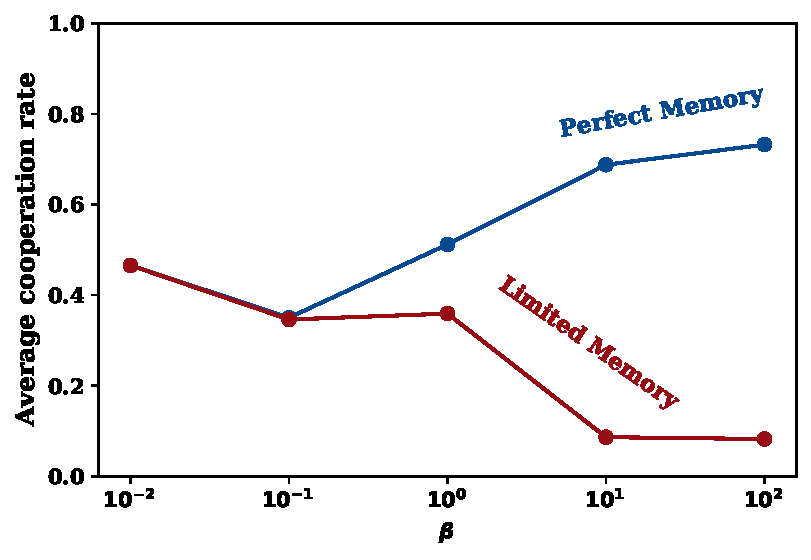
\includegraphics[width=\textwidth]{static/cooperation_rate_over_betas.pdf}
  \end{subfigure}
\caption{{\bf The evolution of cooperation for different selection strength values.} 
We vary the selection strength $\beta$. In all cases, stochastic payoff
evaluation tends to reduce the evolving cooperation rates. ({\bf A}) the
probabilities \(p, q\) for resident population over \(10^7\) time steps for each
\(\beta\) value. ({\bf B}) The cooperation rate within the resident population
(averaged over all games and over all time steps) over \(\beta\).
Unless explicitly varied, the parameters of the simulation are $N\!=\!100$,
$b\!=\!3$, $c\!=\!1$, $\beta\!=\!1$, $\delta\!=\!0.99$. Simulations are run for
$T\!=\!5\times 10^6$ time steps for each parameter
combination.}\label{fig:cooperation_rate_over_betas}
\end{figure}

\subsection{Effect of updating payoffs in different social dilemmas}\label{section:2_by_2_games}

By focusing on the donation game in the previous section, we have gained
insights into the possible effects of the updating payoffs, and how parameters
such as the benefit and the strength of selection might can exaggerate the
effect. However, by focusing on one specific game can narrow our knowledge of
the effects of updating payoffs on the different forms of possible human
interactions and social dilemmas. For this reason we explore not only the 
donation game but all the possible symmetric games. These are given by
Table~\ref{table:social_dilemmas}.

\begin{table}[!htbp]
  \begin{center}
    \resizebox{.6\textwidth}{!}{
    \renewcommand{\arraystretch}{1.5}
      \begin{tabular}{ccc}
  \toprule
  & \textbf{social dilemmas} & \textbf{payoffs' constrains} \\
  \midrule
(i) & stage hunt  & \(R > T > P > S\) \\
(ii) & snowdrift  & \(T > R > S > P\) \\
(iii) & harmony  & \(R > T > S > P\) \\
(iv) & prisoner dilemma  & \(T > R > P > S\) \\
(v)& donation game  & \(T > R > P > S\) \& \(T=b, R=b-c, S=-c, P=0\) \\
  \bottomrule
      \end{tabular}}
  \end{center}
  \caption{\textbf{Social dilemmas and payoffs' constrains}. The various social
  dilemmas we explore in this work. Results for cases (i) - (iv) are presented
  in section~\ref{section:2_by_2_games} and results for case (v) are presented
  in section~\ref{section:donation}.}
  \label{table:social_dilemmas}
\end{table}


% Include discussion on each game?


\begin{figure}
  \centering
  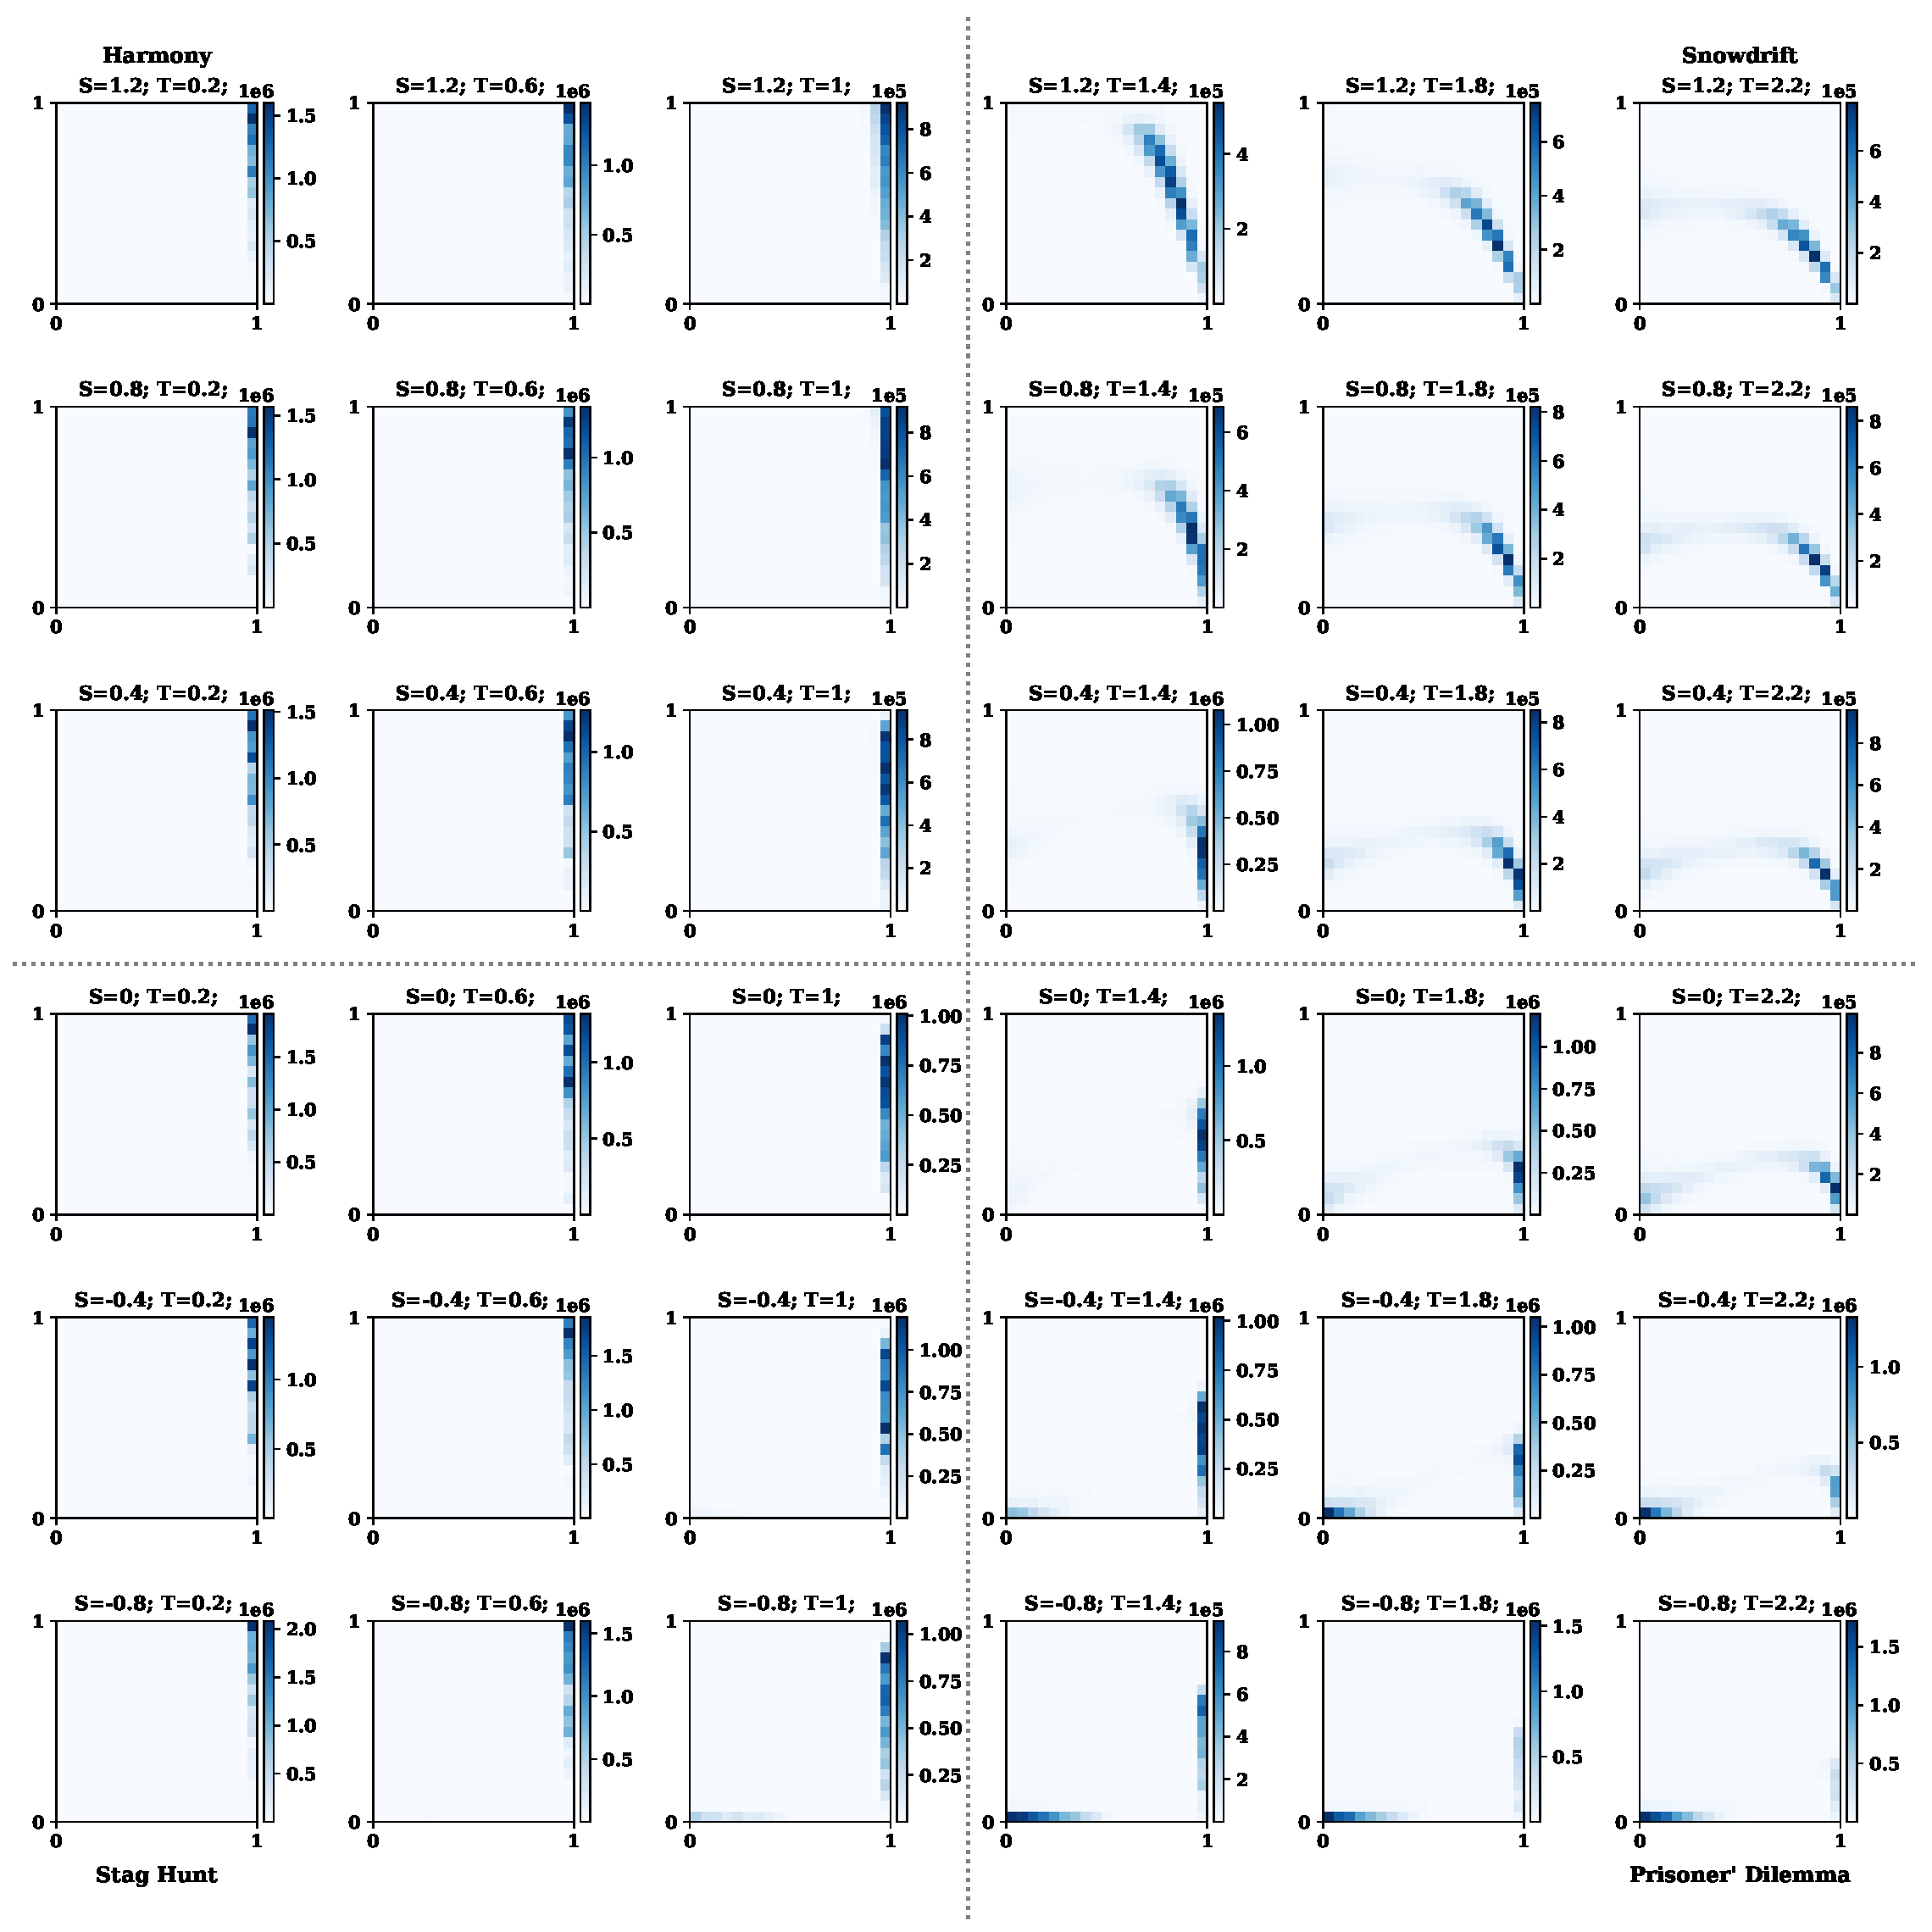
\includegraphics[width=\textwidth]{static/expected_two_by_two_games.pdf}
\end{figure}


\section{Conclusions}\label{section:conclusions}

\appendix

\section{Model Setup}\label{appendix:methods}

Consider a population of \(N\) individuals where \(N\) is even. At any point in
time there are at most two different strategies in present in the population.
More specifically, a mutant strategy played by \(k\) individuals and a resident
strategy played by \(N - k\) individuals. We assume a pairwise process in which
strategies spread because they are imitated more often. Each step of the
evolutionary process consists of two stages; a game stage and an update stage.

In the game stage, each individual is randomly matched with some other
individual in the population. Their interaction lasts for a number of turns
which is not fixed but depends on the continuation probability \(\delta\). At
each turn the individuals choose between cooperation (\(C\)) and defection
(\(D\)). Thus, there are four possible outcomes in each turn \(CC, CD, DC\) and
\(DD\). If both players cooperate they receive the reward payoff \(R\), whereas
if both players defect they receive the punishment payoff \(P\). If one
cooperates but the other defects, the defector receives the temptation to
defect, \(T\), whereas the cooperator receives the sucker's payoff, \(S\).
Let $\mathcal{U}=\{R,S,T,P\}$ denote the set of feasible payoffs in each round,
and let $\mathbf{u}\!=\!(R,S,T,P)$ be the corresponding payoff vector.
The values of the payoffs are not only based on the prisoner's dilemma but all
the symmetric \(2 \times 2\) games, Table~\ref{table:social_dilemmas}.

A further assumption of our model is that individuals make use of reactive
strategies when they make decisions in each round. Reactive strategies are a set
of strategies that take into account only the previous action of the opponent.
A reactive strategy can be written explicitly as a vector,

\[s=(y, p, q)\]

where \(y\) is the probability that the strategy opens with a cooperation and
\(p, q\) are the probabilities that the strategy cooperates given that the
opponent cooperated and defected equivalently.

In the updating stage, two players are randomly drawn from the population, a
`learner' and a `role model'. The learner adopts the role model's strategy
based on the Fermi distribution function, %ToDo add reference

\begin{equation} \label{Eq:rho}
\rho(u_{L}, u_{RM}) = \frac{1}{1\!+\! \exp^{\!-\!\beta (u_{RM}\!-\!u_{L})}}.
\end{equation}

where $u_{L}\!\in\! \mathcal{U}$ is the learner's payoff, $u_{RM}\!\in\!
\mathcal{U}$ is the role model's payoff, and $\beta\!\ge\!0$ is the intensity of
selection.

We iterate this basic evolutionary step until either the mutant strategy goes
extinct, or until it fixes in the population and becomes the new resident
strategy. After either outcome, we set $k$ to $1$ and we introduce a new mutant
strategy which is uniformly chosen from all reactive strategies at random.
Instead of simulating each step of the evolutionary process, we estimate the
probability that a newly introduced mutant fixes~\cite{nowak2004emergence}. This
is defined as the fixation probability of the mutant, and the standard form is
the following,

\begin{equation}\label{eq:appendix_fixation_probability}
\varphi = \frac{1}{1+\sum\limits_{i=1}^{N-1}\prod\limits_k^i \frac{\lambda^-_k}{\lambda^+_k}},
\end{equation}

where \(\lambda^-_k, \lambda^+_k\) are the probabilities that the number of
mutants decreases and increases respectively.

This process of mutation and fixation/extinction is iterated many times. The
evolutionary process is summarized by
Algorithm~\ref{algorithm:pairwise_comparison}.

\begin{algorithm}[!htbp]
  \SetAlgoLined
   $N \leftarrow$ population size\;
   $k \leftarrow 1$\;
   resident $\leftarrow (0, 0, 0)$\;
   \While{step $<$ maximum number of steps}{
    mutant $\leftarrow$ random: $\{\emptyset \}\ \rightarrow R^3$\;
    fixation probability $\leftarrow \varphi $\;
    \If{$\varphi >$ random: $i \rightarrow [0, 1]$}{
      resident $\leftarrow$ mutant;
     }}
     \caption{Evolutionary process}\label{algorithm:pairwise_comparison}
\end{algorithm}

The aim of this work is to explore the effect of updating memory on the
cooperation rate of the evolved population. For this reason we consider two
different approaches when estimating the payoffs at the updating stage. The two
approaches we consider are those of (i) the expected and (ii) the limited memory
payoffs.

\subsection*{Expected Payoffs}

The expected payoffs are the conventional payoffs used in the updating
stage~\cite{imhof2010stochastic}. They are defined as the mean payoff of an
individual in a well-mixed population that engages in repeated games with all
other population members.

We first define the payoff of two reactive strategies at the game stage. Assume
two reactive strategies $s_1\!=\!(y_1, p_1, q_1$) and $s_2\!=\!(y_2,p_2,q_2)$.
It is not necessary to simulate the play move by move, instead the play between
the two strategies is defined a Markov matrix \(M\),

\begin{equation}\label{eq:transition_matrix}
  M = \left[\begin{matrix} p_{1} p_{2} & p_{1} \left(1 - p_{2}\right) & p_{2} \left(1 - p_{1}\right) & \left(1 - p_{1}\right) \left(1 - p_{2}\right)\\
    p_{2} q_{1} & q_{1} \left(1 - p_{2}\right) & p_{2} \left(1 - q_{1}\right) & \left(1 - p_{2}\right) \left(1 - q_{1}\right)\\
    p_{1} q_{2} & p_{1} \left(1 - q_{2}\right) & q_{2} \left(1 - p_{1}\right) & \left(1 - p_{1}\right) \left(1 - q_{2}\right)\\
    q_{1} q_{2} & q_{1} \left(1 - q_{2}\right) & q_{2} \left(1 - q_{1}\right) & \left(1 - q_{1}\right) \left(1 - q_{2}\right)\end{matrix}\right].
\end{equation}

whose stationary vector \(\mathbf{v}\), combined with the payoff \(u\), yields
the game stage outcome for each strategy,
\(\langle\mathbf{v}(s_1,s_2),\mathbf{u}\rangle\)~\cite{Hauert1997}.


In the updating stage the learner adopts the strategy of the role model based on
their updating payoffs. Given that there are only two different types in the
population at each time step we only need to define the expected payoff for a
resident (\(\pi_R\)) and for a mutant (\(\pi_M\)). Assume the resident strategy
\(s_R = (y_R, p_R, q_R)\) and the mutant strategy \(s_M = (y_M, p_M, q_M)\), the
expected payoffs are give by,

\begin{equation} \label{Eq:ExpPay}
  \begin{array}{lcrcr}
  \displaystyle \pi_R	&=	&\displaystyle \frac{N\!-\!k\!-\!1}{N-1}\cdot \langle\mathbf{v}(s_R,s_R),\mathbf{u}\rangle	&+	&\displaystyle\frac{k}{N-1}\cdot \langle\mathbf{v}(s_R,s_M),\mathbf{u}\rangle,\\[0.5cm]
  \displaystyle \pi_M	&=	&\displaystyle\frac{N-k}{N-1}\cdot \langle\mathbf{v}(s_M,s_R),\mathbf{u}\rangle&+	&\displaystyle\frac{k-1}{N-1}\cdot \langle\mathbf{v}(s_M,s_M),\mathbf{u}\rangle.\\
  \end{array}
\end{equation}

The number of mutant in the population increase if a learner resident adopts the
strategy of a mutant role model, and decreases if a mutant leaner adopts the
strategy of a resident. The probabilities that the number of mutants decreases
and increases, \(\lambda^-_k\) and \(\lambda^+_k\), are not explicitly define
as,

\begin{align*} 
  \lambda^-_k &\!=\!\rho(\pi_R, \pi_M) \\
  \lambda^+_k &\!=\!\rho(\pi_M, \pi_R).
\end{align*}

\subsection*{Limited memory payoffs}

Initially, we discuss the case of the last round updating payoff. At the stage
game we define the payoff of a reactive strategy in the last round,
Proposition~\ref{proposition:last_round}.


\begin{Prop}
    Consider a repeated prisoner's dilemma, with
    continuation probability $\delta$, between players with reactive strategies
    $s_1\!=\!(y_1, p_1, q_1$)  and $s_2\!=\!(y_2,p_2,q_2)$ respectively. Then the
    probability that the $s_1$ player receives the payoff $u\!\in\! \mathcal{U}$ in
    the very last round of the game is given by $v_{u}(s_1,s_2)$, as given by
    Equation~(\ref{Eq:LastRound}).

    \begin{equation} \label{Eq:LastRound}
      \setlength{\arraycolsep}{1pt}
      \begin{array}{rcl}
    
      v_{R}(s_1,s_2) &= &\displaystyle (1\!-\!\delta)\frac{y_1y_2}{1\!-\!\delta^2 r_1 r_2}+\delta \frac{\Big(q_1+r_1\big((1\!-\!\delta)y_2+\delta q_2\big)\Big) \Big(q_2+r_2\big((1\!-\!\delta)y_1+\delta q_1\big)\Big)}
      {\displaystyle(1\!-\!\delta r_1r_2)(1\!-\!\delta^2 r_1 r_2)} \times R,\\[1cm]
    
      v_{S}(s_1,s_2) &= &\displaystyle (1\!-\!\delta)\frac{y_1\bar{y}_2}{1\!-\!\delta^2 r_1 r_2}+\delta \frac{\Big(q_1+r_1\big((1\!-\!\delta)y_2+\delta q_2\big)\Big) \Big(\bar{q}_2+\bar{r}_2\big((1\!-\!\delta)y_1+\delta p_1\big)\Big)}
      {\displaystyle(1\!-\!\delta r_1r_2)(1\!-\!\delta^2 r_1 r_2)} \times S,\\[1cm]
    
      v_{T}(s_1,s_2) &= &\displaystyle (1\!-\!\delta)\frac{\bar{y}_1y_2}{1\!-\!\delta^2 r_1 r_2}+\delta \frac{\Big(\bar{q}_1+\bar{r}_1\big((1\!-\!\delta)y_2+\delta p_2\big)\Big) \Big(q_2+r_2\big((1\!-\!\delta)y_1+\delta q_1\big)\Big)}
      {\displaystyle(1\!-\!\delta r_1r_2)(1\!-\!\delta^2 r_1 r_2)} \times T,\\[1cm]
    
      v_{P}(s_1,s_2) &= &\displaystyle (1\!-\!\delta)\frac{\bar{y}_1\bar{y}_2}{1\!-\!\delta^2 r_1 r_2}+\delta \frac{\Big(\bar{q}_1+\bar{r}_1\big((1\!-\!\delta)y_2+\delta p_2\big)\Big) \Big(\bar{q}_2+\bar{r}_2\big((1\!-\!\delta)y_1+\delta p_1\big)\Big)}
      {\displaystyle(1\!-\!\delta r_1r_2)(1\!-\!\delta^2 r_1 r_2)} \times P.
      \end{array}
    \end{equation}

In these expressions, we have used the notation $r_i:=p_i\!-\!q_i$,
$\bar{y}_i\!=\!1\!-\!y_i$, $\bar{q}_i:=1\!-\!q_i$, and
$\bar{r}_i:=\bar{p}_i\!-\!\bar{q}_i=-r_i$ for $i\!\in\!\{1,2\}$.
\end{Prop}

\begin{proof}
Given a play between two reactive strategies with continuation probability
$\delta$. The outcome at turn \(t\) is given by,

\begin{equation}\label{eq:}
  (1 - \delta) \mathbf{v_0} \sum \delta^{t} M^{(t)},
\end{equation}

where $\mathbf{v_0}$ denotes the expected distribution of the four outcomes in
the very first round, and \(1- \delta\) the probability that the game ends.
It can be shown that,

\begin{align*}
  (1 - \delta) \mathbf{v_0} \sum \delta^{t} M^{(t)} & = (1 - \delta)(\mathbf{v_0} + \delta \mathbf{v_0} M + \delta^{2}\mathbf{v_0} M ^{2} + \dots )\\ 
   & = (1 - \delta)\mathbf{v_0} (1 + \delta M + \delta^{2}M ^{2} + \dots ) \text{ using standard formula for geometric series}\\ 
   & = (1 - \delta)\mathbf{v_0}(I_4 - \delta M)^{-1}
\end{align*}

where \((1 - \delta)\mathbf{v_0}(I_4 - \delta M)^{-1}\) is vector \(\in R^{4}\)
and it the probabilities for being in any of the outcomes \(CC, CD, DC, DD\) in
the last round. Combining this with the payoff vector \(u\) and some algebraic
manipulation we derive to the Equation~\ref{Eq:LastRound}.
\end{proof}

In the updating stage we select a mutant and resident to be either the role
model or the learner. Assume the selected mutant. Given that they can interact
with only one other member of the population, they can interact either the
selected resident, another resident or with another mutant. The same is true for
the the selected resident. They can interact with the selected mutant, another
resident, or another mutant. Thus, in each updating stage there are five
possible combinations of pairs. These are illustrated by
Figure~\ref{fig:single_pairs}.

\begin{figure}[!htbp]
  \centering
  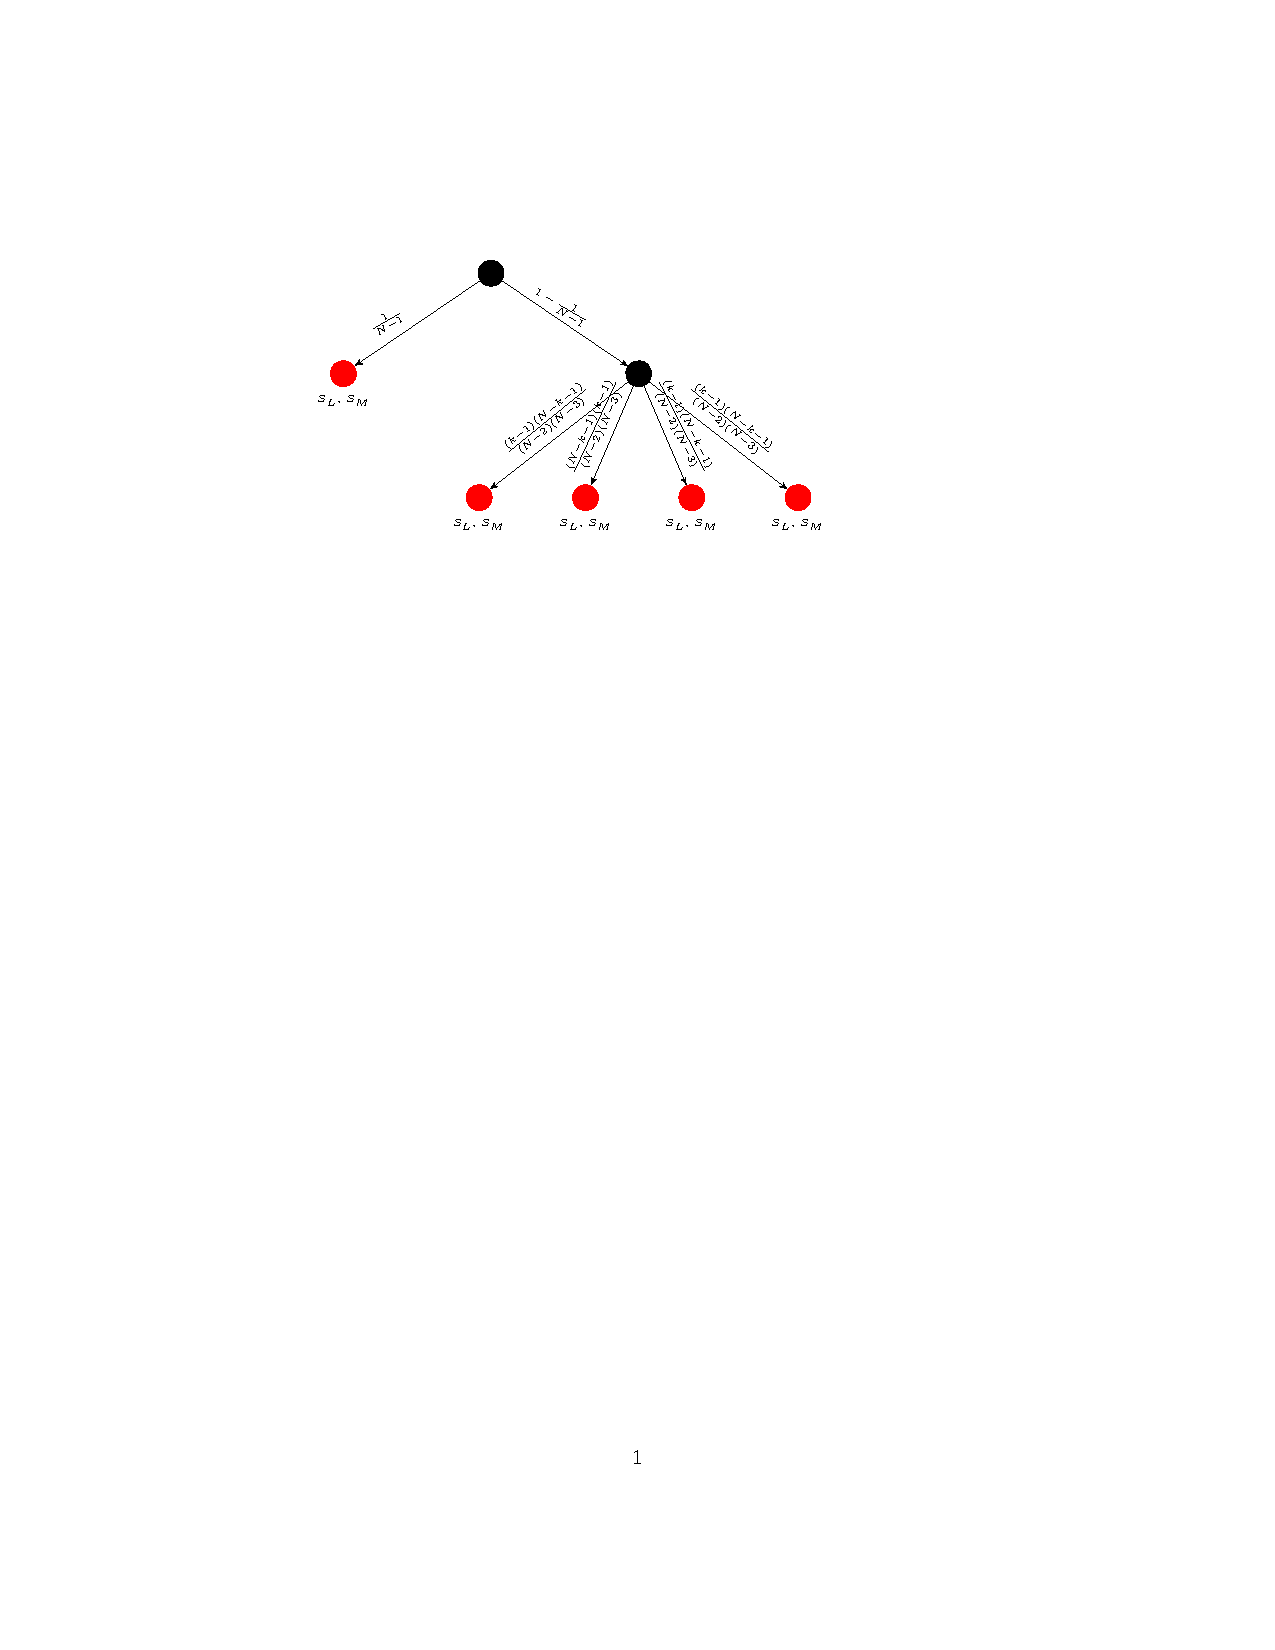
\includegraphics[width=.65\textwidth]{static/last_rounds_matches.tex}
  \caption{\textbf{Possible pairings combination in the updating stage, given
  that individuals interact with only one other member in the population.}. We
  distinguish between the selected resident and the rest of the residents and we
  do the same with the mutants. There is a probability that the selected
  resident interacts with the selected mutant.}\label{fig:single_pairs}
\end{figure}

The probability that the respective payoffs of the players
are given by $u_1$ and $u_2$ can be calculated as

\begin{equation}\label{eq:Chi}
\setlength{\arraycolsep}{1pt}
\begin{array}{llrl}
x(u_1,u_2)	 &=&\displaystyle \frac{1}{N\!-\!1}\cdot  &v_{u_1}(S_1,S_2)\cdot 1_{(u_1,u_2)\in \mathcal{U}^2_F}\\[0.5cm]
&+	
&\displaystyle \left(1\!-\!\frac{1}{N\!-\!1}\right)  
&\left[ \frac{k\!-\!1}{N\!-\!2}\frac{k\!-\!2}{N\!-\!3} v_{u_1}(S_1,S_2) v_{u_2}(S_2,S_2) + 
 \frac{k\!-\!1}{N\!-\!2}\frac{N\!-\!k\!-\!1}{N\!-\!3} v_{u_1}(S_1,S_2) v_{u_2}(S_2,S_1)\right.\\[0.5cm]
&&&\left. +\frac{N\!-\!k\!-\!1}{N\!-\!2}\frac{k\!-\!1}{N\!-\!3} v_{u_1}(S_1,S_1) v_{u_2}(S_2,S_2) + 
 \frac{N\!-\!k\!-\!1}{N\!-\!2}\frac{N\!-\!k\!-\!2}{N\!-\!3} v_{u_1}(S_1,S_1) v_{u_2}(S_2,S_1)\right].
\end{array}
\end{equation}

The first term on the right side corresponds to the case that the learner and
the role model happened to be matched during the game stage, which happens with
probability $1/(N\!-\!1)$.In that case, we note that only those payoff pairs
can occur that are feasible in a direct interaction, $\splitatcommas{(u_1,u_2)\in
\mathcal{U}^2_F:=\big\{ (R,R), (S,T), (T,S), (P,P) \big\}}$, as represented by
the respective indicator function. Otherwise, if the learner and the role model
did not interact directly, we need to distinguish four different cases,
depending on whether the learner was matched with a resident or a mutant, and
depending on whether the role model was matched with a resident or a mutant.

Given that $N\!-\!k$ players use the resident strategy $S_1\!=\!(y_1,p_1,q_1)$
and that the remaining $k$ players use the mutant strategy
$S_2\!=\!(y_2,p_2,q_2)$, the probability that the number of mutants increases by
one in one step of the evolutionary process can be written as

\begin{align}
\lambda^+_k=\frac{N\!-\!k}{N}\cdot \frac{k}{N}\cdot \sum_{u_1,u_2\in\mathcal{U}} x(u_1,u_2)\cdot \rho(u_1,u_2), \\
\lambda^-_k=\frac{N\!-\!k}{N}\cdot \frac{k}{N}\cdot \sum_{u_1,u_2\in\mathcal{U}} x(u_1,u_2)\cdot \rho(u_2,u_1).
\end{align}

In this expression, $(N\!-\!k)/N$ is the probability that the randomly chosen
learner is a resident, and $k/N$ is the probability that the role model is a
mutant. The sum corresponds to the total probability that the learner adopts the
role model's strategy over all possible payoffs $u_1$ and $u_2$ that the two
player may have received in their respective last rounds. We use $x(u_1,u_2)$ to
denote the probability that the randomly chosen resident obtained a payoff of
$u_1$ in the last round of his respective game, and that the mutant obtained a
payoff of $u_2$.

This framework can be extended to consider the case of where the payoffs
correspond to the last \(n\) rounds payoff an individual achieved after
interacting with \(m\) other individuals. For the case \(n=2\) the payoffs
at the game stage are,

\begin{Prop}\label{proposition:last_two_rounds}
Assume a play between the reactive strategies \(s_1\) and \(s_2\) with a
continuation probability \(\delta\). Then the probability of being in any of the
sixteen outcomes \(\splitatcommas{RR, RR, RR, RR, RR, RR, RR, RR, RR, RR, RR, RR, RR, RR, RR, RR}\)
on the last two rounds are given by,

\begin{equation}
  \mathbf{v_{a_1, a_2}} = (1 - \delta) m_{a_1, a_2} \delta^2 \left[\mathbf{v_0}(I_4 - \delta M)^{-1}\right]_{a_1, a_2}, \quad \text{ for } m_{a_1, a_2} \in M \ \& \ a_1, a_2 \in \{R, S, T, P\}
\end{equation}

\end{Prop}

Proposition~\ref{proposition:last_two_rounds} can be extended to the last \(n\)
rounds.

\begin{Prop}\label{proposition:last_n_rounds}
Assume a play between the reactive strategies \(s_1\) and \(s_2\) with a
continuation probability \(\delta\). Then the probability of being in any of the
sixteen outcomes \(\splitatcommas{RR, RR, RR, RR, RR, RR, RR, RR, RR, RR, RR, RR, RR, RR, RR, RR}\)
on the last two rounds are given by,

\begin{equation}
  \mathbf{v_{a_1, a_2}} = (1 - \delta) \prod m_{a_1, a_2} \delta^2 \left[\mathbf{v_0}(I_4 - \delta M)^{-1}\right]_{a_1, a_2}
\end{equation}

for \(m_{a_1, a_2} \in M\) and \(a_1, a_2 \in [1, 4]\).
\end{Prop}

Equation~\ref{eq:Chi} can also be extended to include interactions with two other
individuals. The possible pairings are illustrated by Figure~\ref{}.


\begin{figure}[!htbp]
  \centering
  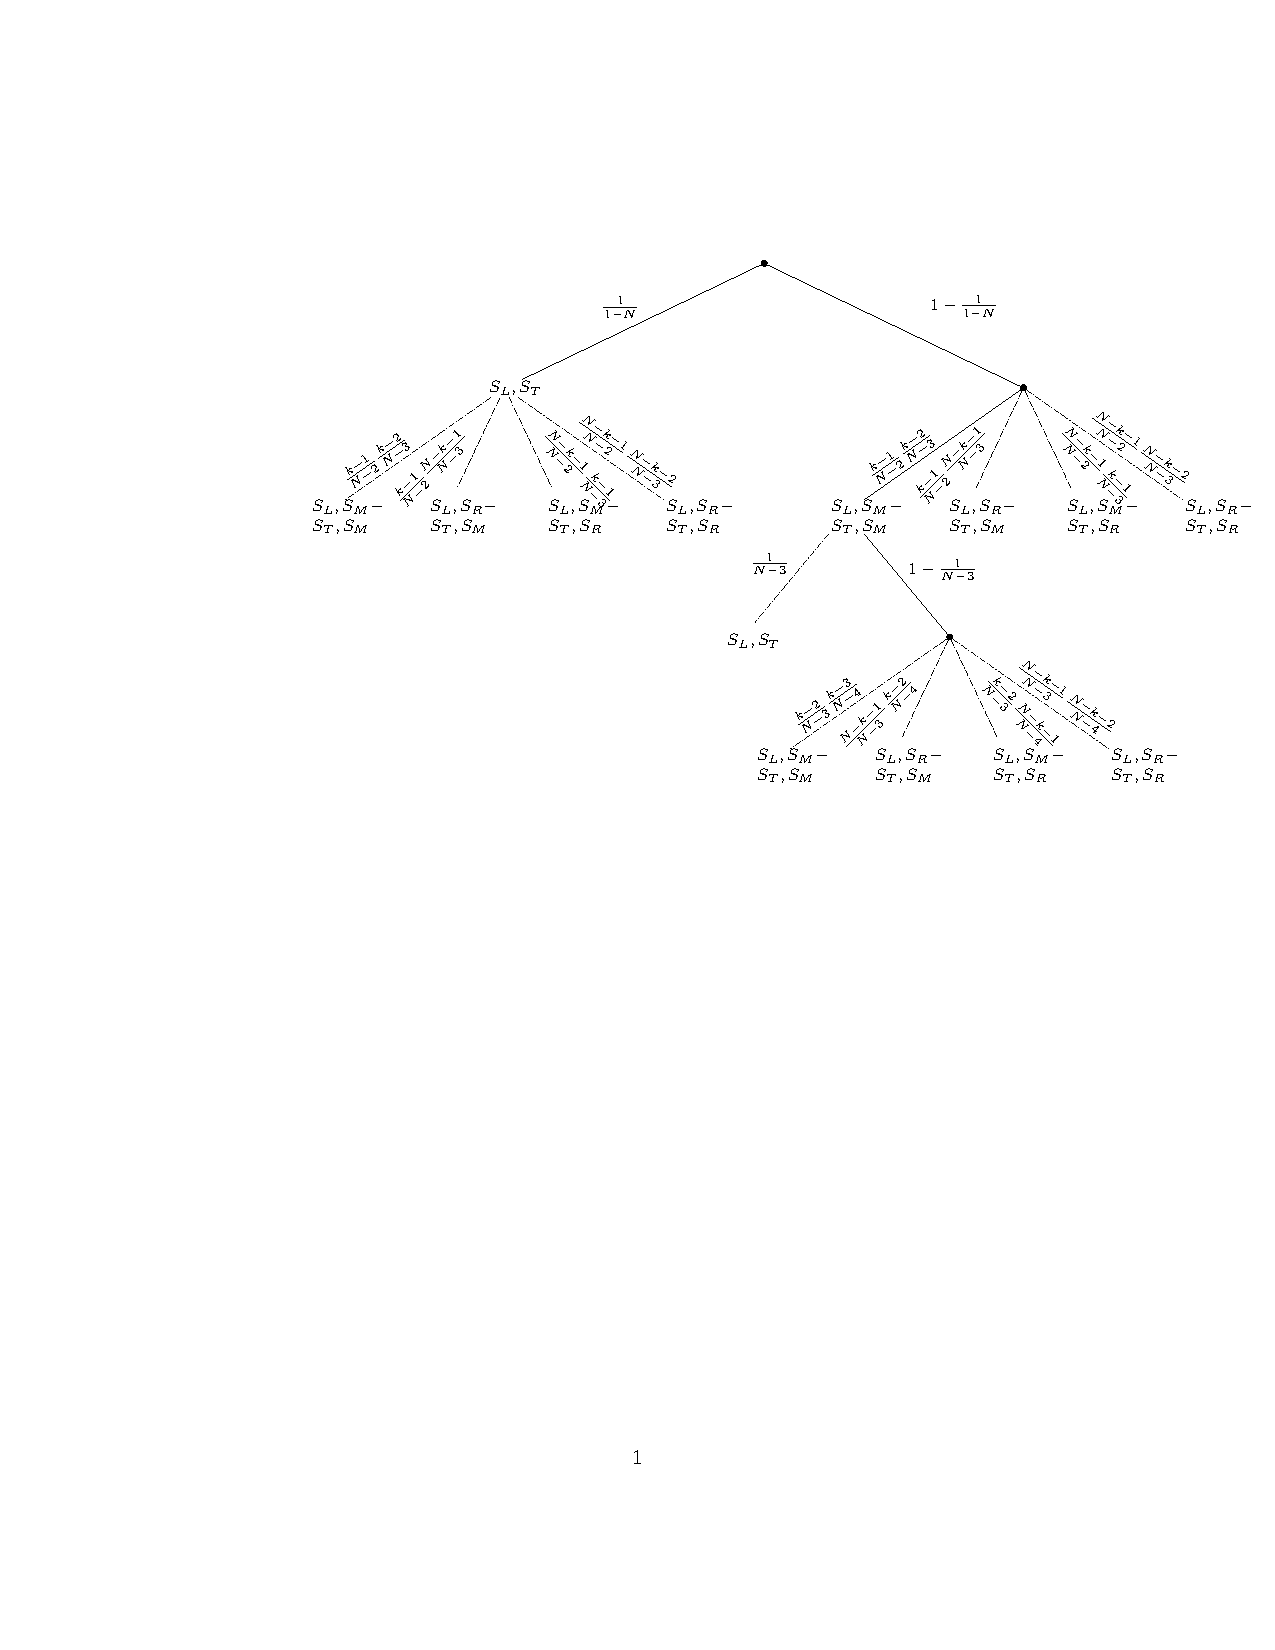
\includegraphics[width=.65\textwidth]{static/tree.tex}
  \caption{The tree}\label{fig:two_pairs}
\end{figure}


\section{Verifying analytical results with simulations}

The analytical results presented in this work have been verified with simulations.
More specifically the probabilities of Equation~(\ref{Eq:LastRound}),

\begin{figure}[!htbp]
  \centering
  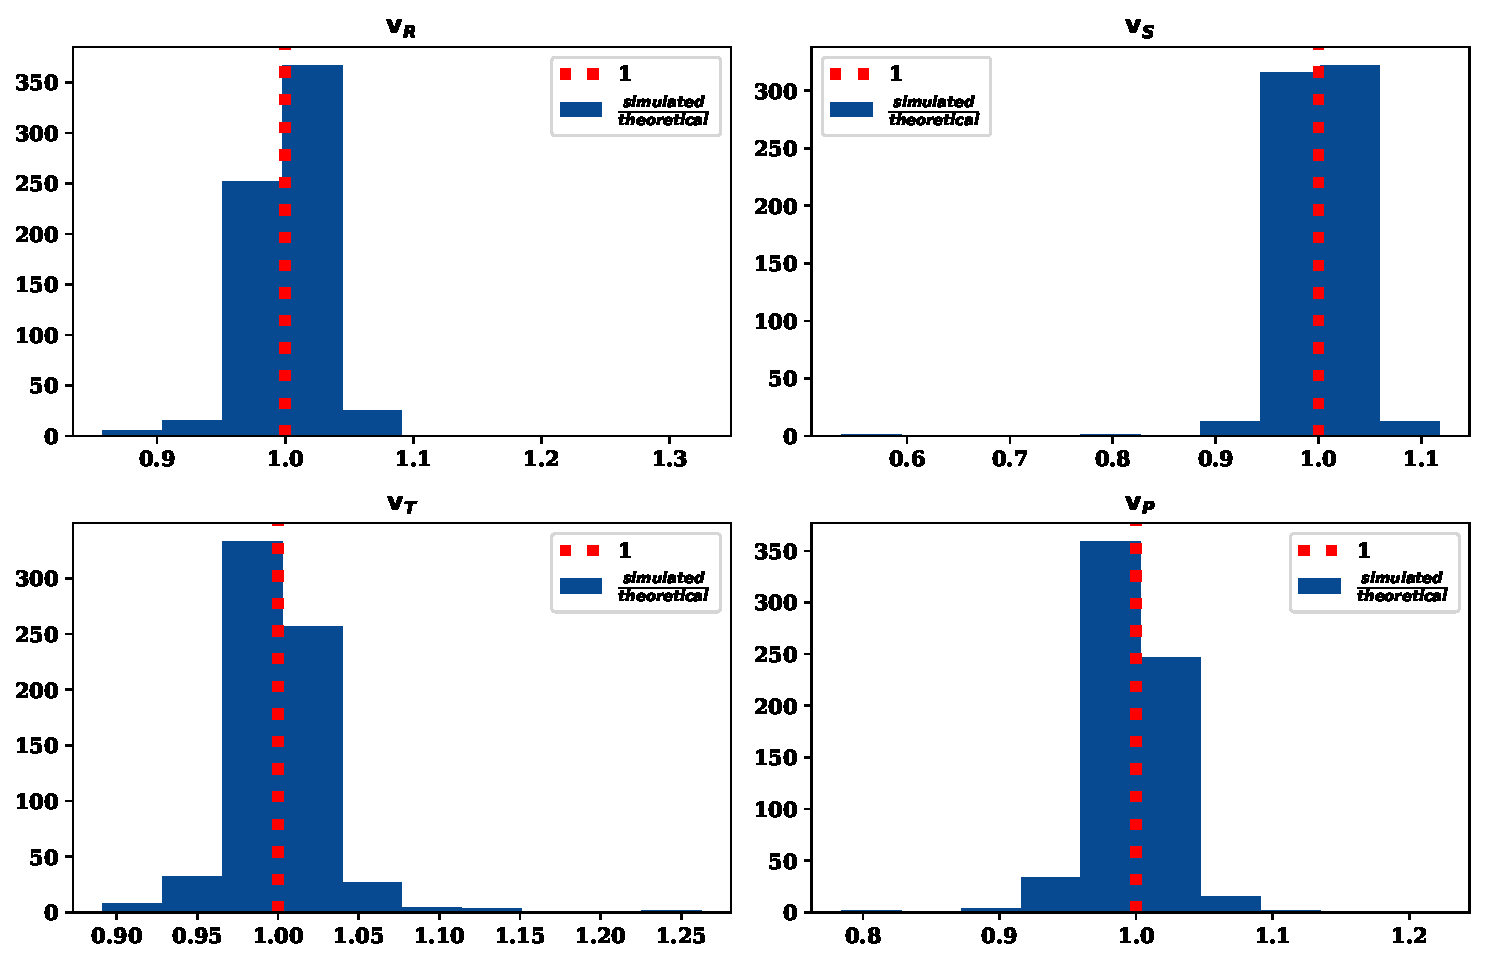
\includegraphics[width=.75\textwidth]{static/stationary_four.pdf}
\caption{}
\end{figure}

Proposition~\ref{proposition:last_two_rounds},

\begin{figure}[!htbp]
  \centering
  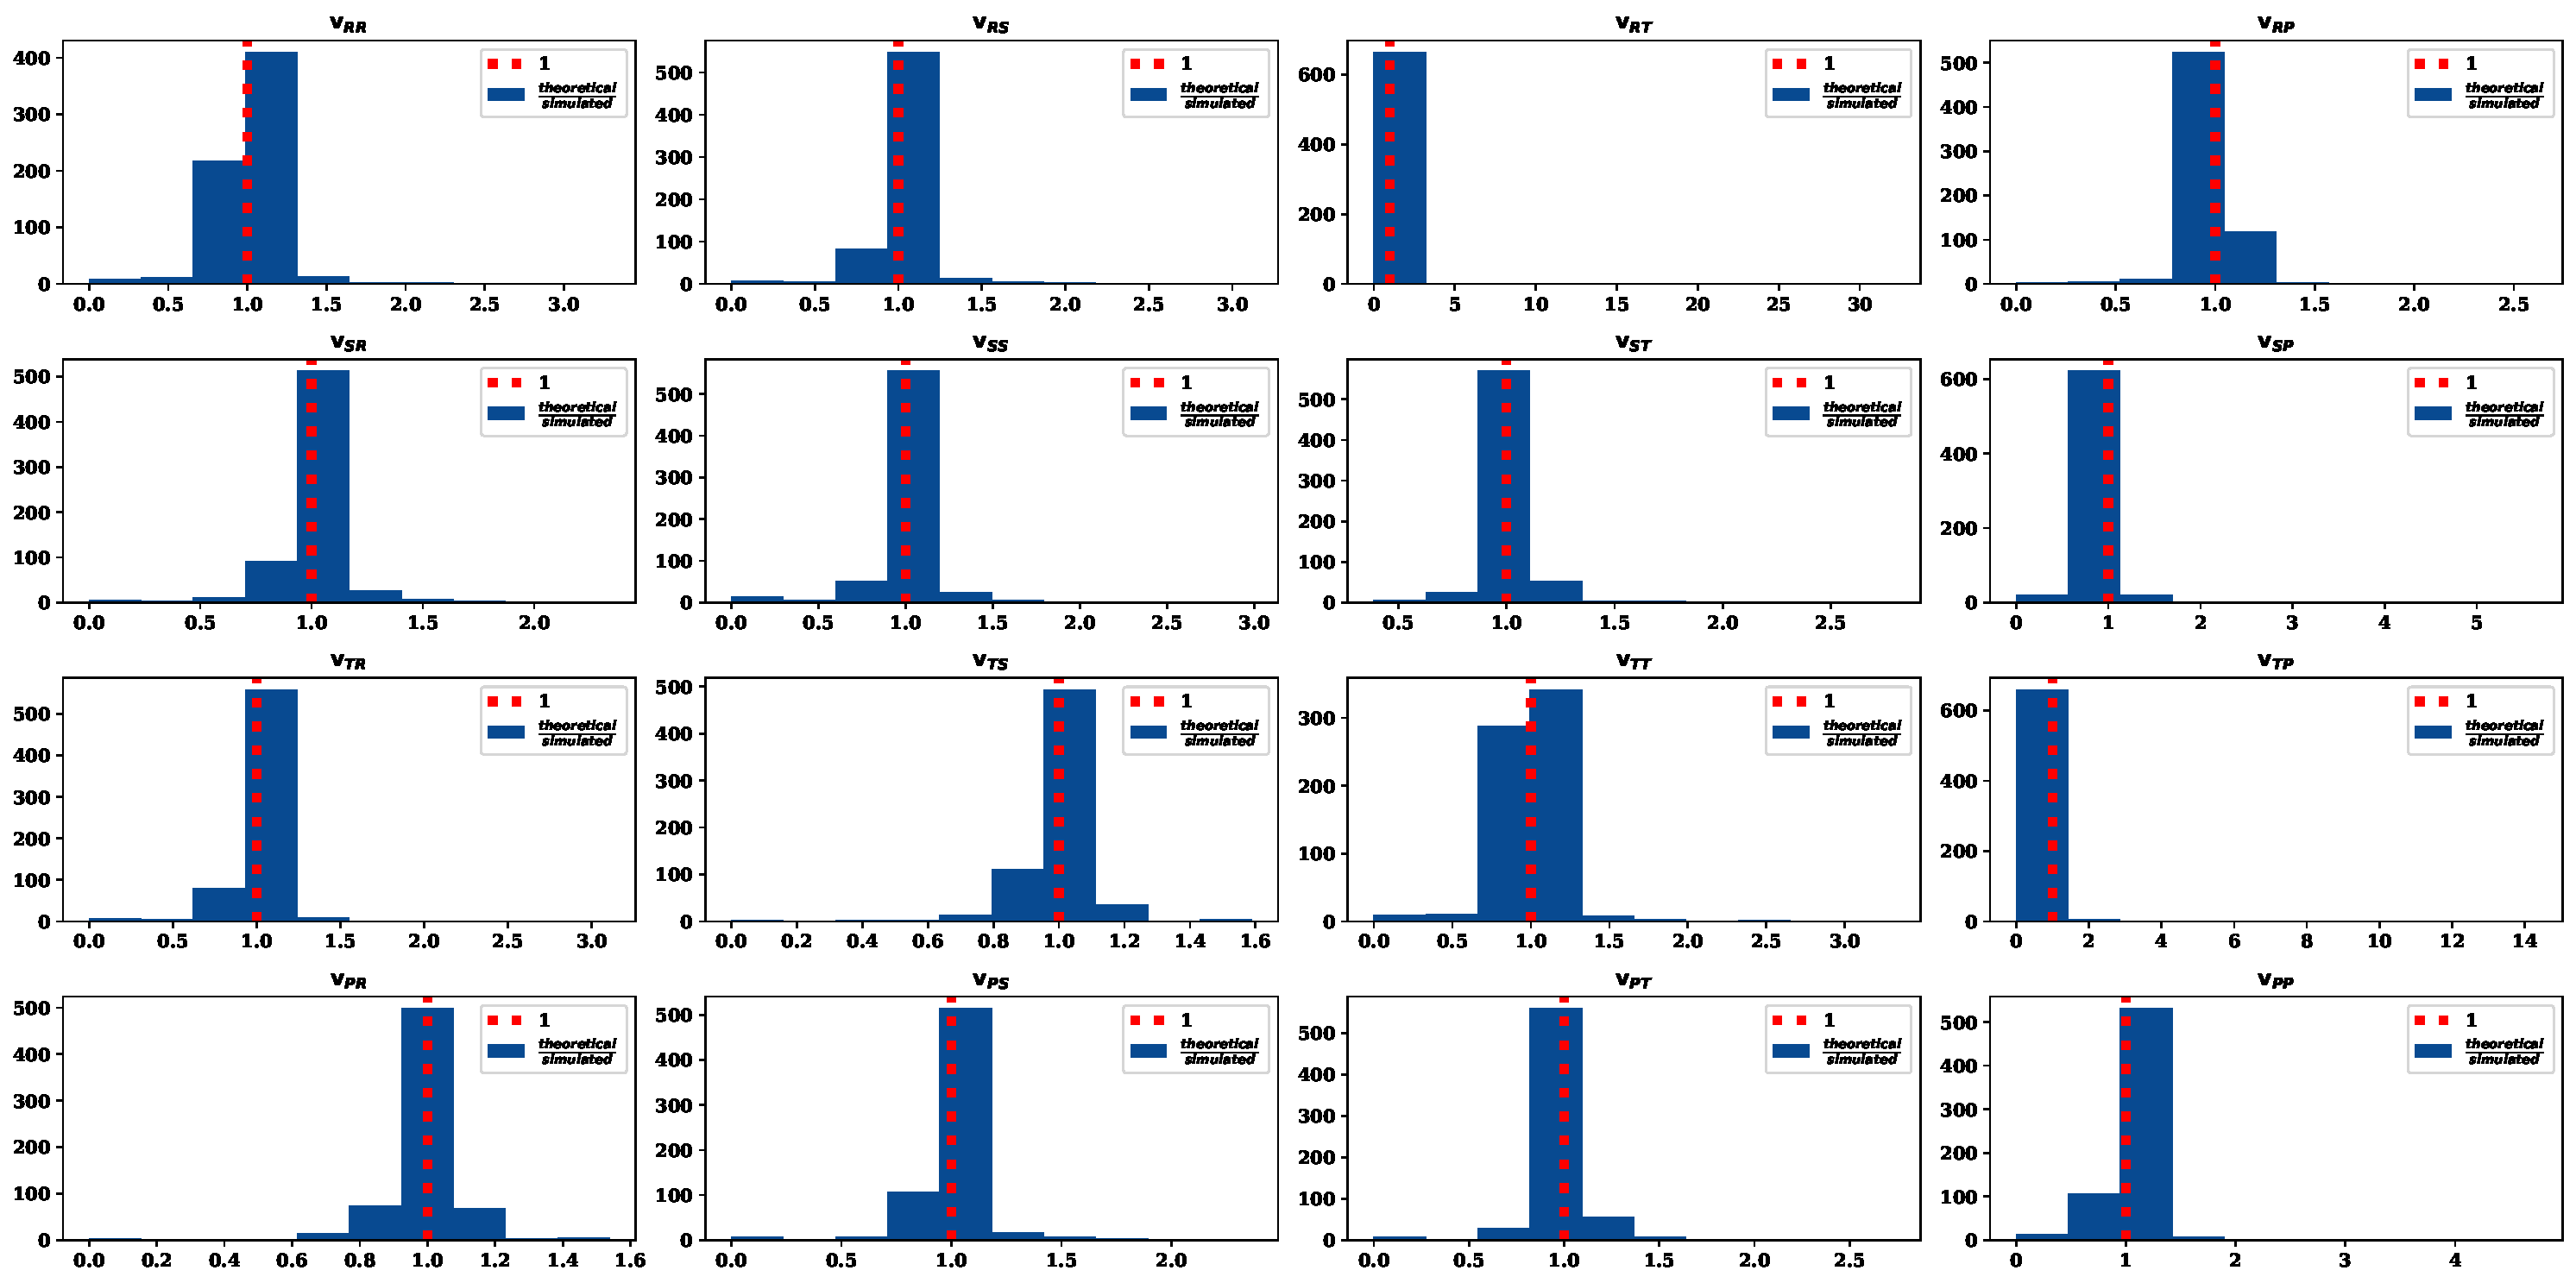
\includegraphics[width=\textwidth]{static/stationary_sixteen.pdf}
\caption{}
\end{figure}



% \begin{Prop}\label{proposition:last_n_rounds}

% \end{Prop}

% \section{Evolutionary dynamics in finite population}

% The Prisoner's Dilemma (PD) is a two player no-cooperative game. The players
% simultaneously and independently make a decision to Cooperate (C) or to defect
% (D). The payoffs for both players depend on their actions and the actions of
% their opponents. More specifically, the payoffs are given by:

% \begin{equation}\label{eq:pd_normal_form}
%     \begin{pmatrix}
%         R & S  \\
%         T & P
%     \end{pmatrix}
% \end{equation}

% The payoffs, \((R, P, S, T)\), are constrained by \(T > R > P > S\) and \(2R > T + S\).

% A special case is the donation game,” where each player can cooperate by providing 
% a benefit \(b\) to the other player at their cost \(c\), with \(0 < c < b\).
% Then, \(T=b, R=b-c, S=-c, P=0\), and matrix~(\ref{eq:pd_normal_form}) is give by:

% \begin{equation}\label{eq:donation_normal_form}
%     \begin{pmatrix}
%         b-c & -c  \\
%         b & 0
%     \end{pmatrix}
% \end{equation}

% where \(c\) is the cost inflicted to an individual for cooperating and \(b\) is
% the benefit.

% The questions of evolution become more interesting when repetition is considered,
% and the history can be accessed when making decisions. The iterated form of the
% game is called the Iterated Prisoner's Dilemma (IPD). There are several two
% player repeated games such as the Snowdrift game~\cite{sugden2004economics},
% Harmony and the Stag Hunt~\cite{skyrms2001stag} game. We present results in all
% four games.

% The space of strategies in the IPD is infinite. To continue with our
% evolutionary analysis, we assume herein that individuals at most make use of
% simple \textbf{reactive strategies}. Reactive strategy are a set of memory-one
% strategies that only take into account the previous action of the opponent. An
% example of a reactive strategy is Tit For Tat. Reactive strategies can be
% written explicitly as a vector \(\in \R_{3}\). More specifically a reactive
% strategy \(s\) is given by \(s=(y, p, q)\) where \(y\) is the probability that
% the strategy opens with a cooperation and \(p, q\) are the probabilities that
% the strategy cooperates given that the opponent cooperated and defected
% equivalently.

% A match between two reactive strategies takes the form of a stochastic process,
% and more specifically, of a Markov chain with four possible states \(CC, CD, DC,
% DD\) (the possible outcomes of each round). We assume a match between two
% reactive strategies \(s_{1}=(y_{1}, p_{1}, q_{1})\) and \(s_{2}=(y_{2}, p_{2},
% q_{2})\), the Markov process is described by the transition matrix \(M\):

% \begin{equation}
%     M = \left[\begin{matrix} p_{1} p_{2} & p_{1} \left(1 - p_{2}\right) & p_{2} \left(1 - p_{1}\right) & \left(1 - p_{1}\right) \left(1 - p_{2}\right)\\
    p_{2} q_{1} & q_{1} \left(1 - p_{2}\right) & p_{2} \left(1 - q_{1}\right) & \left(1 - p_{2}\right) \left(1 - q_{1}\right)\\
    p_{1} q_{2} & p_{1} \left(1 - q_{2}\right) & q_{2} \left(1 - p_{1}\right) & \left(1 - p_{1}\right) \left(1 - q_{2}\right)\\
    q_{1} q_{2} & q_{1} \left(1 - q_{2}\right) & q_{2} \left(1 - q_{1}\right) & \left(1 - q_{1}\right) \left(1 - q_{2}\right)\end{matrix}\right]
% \end{equation}

% The long run steady state probability vector \(\mathbf{v}\), which is the
% solution to \(\mathbf{v} M = \mathbf{v}\), can be combined with the payoff of
% matrix (\ref{eq:pd_normal_form}) (denoted as \(U\)) to give the expected payoffs
% for each player. More specifically, the payoffs for a reactive strategy \(s_1\)
% against an opponent \(s_2\) is:

% \begin{equation}
%     \mathbf{v}(s_1, s_2) \cdot U
% \end{equation}

% where

% \begin{equation}
%     U = \{R, S, T, P\}.
% \end{equation}

% \subsection{Evolutionary Dynamics}

% In evolution context we consider a population of \(N\) players,
% where \(N\) is even, and where mutations are sufficiently rare. At any point
% in time the there are at most two different strategies are present in
% the population. Suppose there are \(N - k\) players who use the strategy \(s_{1}=(y_{1},
% p_{1}, q_{1})\), whereas \(k\) players use the strategy \(s_{2}=(y_{2}, p_{2},
% q_{2})\). We refer to these two player types as ‘residents’ and ‘mutants’,
% respectively.

% Each step of the evolutionary process consists of two stages, a game stage and
% an updating stage.

% \begin{enumerate}
%     \item In the game stage, each player is randomly matched with some
%     other player in the population to interact in one instance of the IPD.
%     \item In the updating stage, two players are randomly drawn from
%     the population, a `learner' and a `exemplar'. Given that the learner's payoff
%     in the last round is $u_L\!\in\! \mathcal{U}$ and that the exemplar's last
%     round's payoff $u_E\!\in\! \mathcal{U}$, we assume the learner adopts the role
%     model's strategy with probability 

%     \begin{equation} \label{Eq:rho}
%     \rho(u_L, u_E) = \frac{1}{1\!+\!\exp\big[ \!-\!\beta (u_E\!-\!u_L) \big]}. 
%     \end{equation}

%     where $\beta\!\ge\!0$ corresponds to the strength of selection.
% \end{enumerate}

% We iterate this basic evolutionary step until either the mutant strategy goes
% extinct, or until it fixes in the population (in which case the mutant strategy
% becomes the new resident strategy). After either outcome, we introduce a new
% mutant strategy $s'_2\!=\!(y_2',p_2',q_2')$ (uniformly chosen from all reactive
% strategies at random), and we set the number of mutants to $k\!=\!1$. This
% process of mutation and fixation/extinction is then iterated many times.

% We compare this process for what we defined as {\bf stochastic payoff
% evaluation} with the analogous process where players update their strategies
% with respect to their {\bf expected} payoffs,

% \begin{equation} \label{eq:ExpPay}
% \begin{array}{lcrcr}
% \pi_1 &= &\displaystyle \frac{N\!-\!k\!-\!1}{N-1}\cdot \langle\mathbf{v}(s_1,s_1),\mathbf{U}\rangle	& + &\displaystyle\frac{k}{N-1}\cdot \langle\mathbf{v}(s_1,s_2),\mathbf{U}\rangle,\\[0.5cm]
% \pi_2 &= &\displaystyle\frac{N-k}{N-1}\cdot \langle\mathbf{v}(s_2,s_1),\mathbf{U}\rangle & + &\displaystyle\frac{k-1}{N-1}\cdot \langle\mathbf{v}(s_2,s_2),\mathbf{U}\rangle.\\
% \end{array}
% \end{equation}

% In the limit of no discounting, $\delta\!\rightarrow\! 1$, this process based on
% expected payoffs has been considered in~\cite{imhof2010stochastic}.

% \subsection{Stochastic payoff evaluation}

% We define {\bf stochastic payoff} as the average payoff $u\!\in\! \mathcal{U}$ a player
% receives in the last \(n\) rounds of the game given that they interact with
% \(m\) players.

% \subsubsection*{Case \(n=m=1\).}

% Initially, consider the situation where \(n=m=1\). The player's stochastic
% payoff is what they receive in the last round against a single opponent. There
% only four possible outcomes for the last round, those are \(CC, CD, DC, DD\).
% Consider two players with reactive strategies $S_1\!=\!(y_1, p_1, q_1$) and
% $S_2\!=\!(y_2,p_2,q_2)$ who interact in a repeated prisoner's dilemma with
% continuation probability $\delta$, the probability that are in each of the
% four possible states in the last round is given by:

% \begin{equation}
%     \mathbf{v}(s_1,s_2)\!=\!\Big(\mathbf{v}_{R}(s_1,s_2),\mathbf{v}_{S}(s_1,s_2),\mathbf{v}_{T}(s_1,s_2),\mathbf{v}_{P}(s_1,s_2)\Big).
% \end{equation}

% where,

% \begin{equation} \label{Eq:LastRound}
%     \setlength{\arraycolsep}{1pt}
%     \begin{array}{rcl}

%     \mathbf{v}_{R}(S_1,S_2) &= &\displaystyle (1\!-\!\delta)\frac{y_1y_2}{1\!-\!\delta^2 r_1 r_2}+\delta \frac{\Big(q_1+r_1\big((1\!-\!\delta)y_2+\delta q_2\big)\Big) \Big(q_2+r_2\big((1\!-\!\delta)y_1+\delta q_1\big)\Big)}
%     {\displaystyle(1\!-\!\delta r_1r_2)(1\!-\!\delta^2 r_1 r_2)},\\[1cm]

%     \mathbf{v}_{S}(S_1,S_2) &= &\displaystyle (1\!-\!\delta)\frac{y_1\bar{y}_2}{1\!-\!\delta^2 r_1 r_2}+\delta \frac{\Big(q_1+r_1\big((1\!-\!\delta)y_2+\delta q_2\big)\Big) \Big(\bar{q}_2+\bar{r}_2\big((1\!-\!\delta)y_1+\delta p_1\big)\Big)}
%     {\displaystyle(1\!-\!\delta r_1r_2)(1\!-\!\delta^2 r_1 r_2)},\\[1cm]

%     \mathbf{v}_{T}(S_1,S_2) &= &\displaystyle (1\!-\!\delta)\frac{\bar{y}_1y_2}{1\!-\!\delta^2 r_1 r_2}+\delta \frac{\Big(\bar{q}_1+\bar{r}_1\big((1\!-\!\delta)y_2+\delta p_2\big)\Big) \Big(q_2+r_2\big((1\!-\!\delta)y_1+\delta q_1\big)\Big)}
%     {\displaystyle(1\!-\!\delta r_1r_2)(1\!-\!\delta^2 r_1 r_2)},\\[1cm]

%     \mathbf{v}_{P}(S_1,S_2) &= &\displaystyle (1\!-\!\delta)\frac{\bar{y}_1\bar{y}_2}{1\!-\!\delta^2 r_1 r_2}+\delta \frac{\Big(\bar{q}_1+\bar{r}_1\big((1\!-\!\delta)y_2+\delta p_2\big)\Big) \Big(\bar{q}_2+\bar{r}_2\big((1\!-\!\delta)y_1+\delta p_1\big)\Big)}
%     {\displaystyle(1\!-\!\delta r_1r_2)(1\!-\!\delta^2 r_1 r_2)}.
%     \end{array}
% \end{equation}

% \begin{proof}

% Assume a repeated prisoner's dilemma between two reactive strategies. Given the
% continuation probability $\delta$, probability that the game ends in the after
% the first round $(1 - \delta)$ and the expected distribution of the four
% outcomes in the very first round is $\mathbf{v_0}$ defined as. Following the
% first round the, the outcome of the next rounds with a probability $\delta$
% is \(M\) such that,

% \[\dots\]

% It can shown that, \(!(1\!-\!\delta)\mathbf{v_0}(I_4-\delta M)^{-1}\) and with
% some algebraic manipulation we derive to Equation~\ref{Eq:LastRound}.

% \end{proof}

% % \begin{Prop}
% %     Consider a repeated prisoner's dilemma, with
% %     continuation probability $\delta$, between players with reactive strategies
% %     $s_1\!=\!(y_1, p_1, q_1$)  and $s_2\!=\!(y_2,p_2,q_2)$ respectively. Then the
% %     probability that the $s_1$ player receives the payoff $u\!\in\! \mathcal{U}$ in
% %     the very last round of the game is given by $v_{u}(S_1,S_2)$, as given by
% %     Eq.~(\ref{Eq:LastRound}).
% % \end{Prop}

% is given by $v_{u}(S_1,S_2)$

% Consider two players with reactive strategies $S_1\!=\!(y_1, p_1, q_1$) and $S_2\!=\!(y_2,p_2,q_2)$ who interact in a repeated prisoner's dilemma with continuation probability $\delta$. We consider the vector 

% \begin{equation}
% \mathbf{v}(S_1,S_2)\!=\!\Big(v_{R}(S_1,S_2),v_{S}(S_1,S_2),v_{T}(S_1,S_2),v_{P}(S_1,S_2)\Big)\!:=\!(1\!-\!\delta)\mathbf{v_0}(I_4-\delta M)^{-1}.
% \end{equation}

% Here, $\mathbf{v_0}$ denotes the expected distribution of the four outcomes in the very first round, $I_4$ is the $4\!\times\!4$ identity matrix, and $M$ is the transition matrix of the Markov chain. 
% The entries of $\mathbf{v}$ can be calculated explicitly,

% \begin{equation} \label{Eq:LastRound}
% \setlength{\arraycolsep}{1pt}
% \begin{array}{rcl}

% v_{R}(S_1,S_2)	&=	&\displaystyle (1\!-\!\delta)\frac{y_1y_2}{1\!-\!\delta^2 r_1 r_2}+\delta \frac{\Big(q_1+r_1\big((1\!-\!\delta)y_2+\delta q_2\big)\Big) \Big(q_2+r_2\big((1\!-\!\delta)y_1+\delta q_1\big)\Big)}
% {\displaystyle(1\!-\!\delta r_1r_2)(1\!-\!\delta^2 r_1 r_2)},\\[1cm]

% v_{S}(S_1,S_2)	&=	&\displaystyle (1\!-\!\delta)\frac{y_1\bar{y}_2}{1\!-\!\delta^2 r_1 r_2}+\delta \frac{\Big(q_1+r_1\big((1\!-\!\delta)y_2+\delta q_2\big)\Big) \Big(\bar{q}_2+\bar{r}_2\big((1\!-\!\delta)y_1+\delta p_1\big)\Big)}
% {\displaystyle(1\!-\!\delta r_1r_2)(1\!-\!\delta^2 r_1 r_2)},\\[1cm]

% v_{T}(S_1,S_2)	&=	&\displaystyle (1\!-\!\delta)\frac{\bar{y}_1y_2}{1\!-\!\delta^2 r_1 r_2}+\delta \frac{\Big(\bar{q}_1+\bar{r}_1\big((1\!-\!\delta)y_2+\delta p_2\big)\Big) \Big(q_2+r_2\big((1\!-\!\delta)y_1+\delta q_1\big)\Big)}
% {\displaystyle(1\!-\!\delta r_1r_2)(1\!-\!\delta^2 r_1 r_2)},\\[1cm]

% v_{P}(S_1,S_2)	&=	&\displaystyle (1\!-\!\delta)\frac{\bar{y}_1\bar{y}_2}{1\!-\!\delta^2 r_1 r_2}+\delta \frac{\Big(\bar{q}_1+\bar{r}_1\big((1\!-\!\delta)y_2+\delta p_2\big)\Big) \Big(\bar{q}_2+\bar{r}_2\big((1\!-\!\delta)y_1+\delta p_1\big)\Big)}
% {\displaystyle(1\!-\!\delta r_1r_2)(1\!-\!\delta^2 r_1 r_2)}.

% %x_1(S_1,S_2)&=&\displaystyle\frac{(1\!-\!\delta)y_1+\delta\Big(q_1+r_1\big((1\!-\!\delta)y_2+\delta q_2\big)\Big)}{1-\delta^2r_1r_2}\\[0.7cm]
% %x_2(S_1,S_2)&=&\displaystyle\frac{(1\!-\!\delta)y_2+\delta\Big(q_2+r_2\big((1\!-\!\delta)y_1+\delta q_1\big)\Big)}{1-\delta^2r_1r_2}.\\
% \end{array}
% \end{equation}

% In these expressions, we have used the notation $r_i:=p_i\!-\!q_i$,
% $\bar{y}_i\!=\!1\!-\!y_i$, $\bar{q}_i:=1\!-\!q_i$, and
% $\bar{r}_i:=\bar{p}_i\!-\!\bar{q}_i=-r_i$ for $i\!\in\!\{1,2\}$. Let
% $\mathcal{U}=\{R,S,T,P\}$ denote the set of feasible payoffs in each round,
% and let $\mathbf{u}\!=\!(R,S,T,P)$ be the corresponding payoff vector. Then
% one can show the following result.

% \includestandalone[width=0.35\textwidth]{static/expected_stochastic}

% \includestandalone{static/stochastic}

% \begin{figure}[!htbp]
%     \centering
%     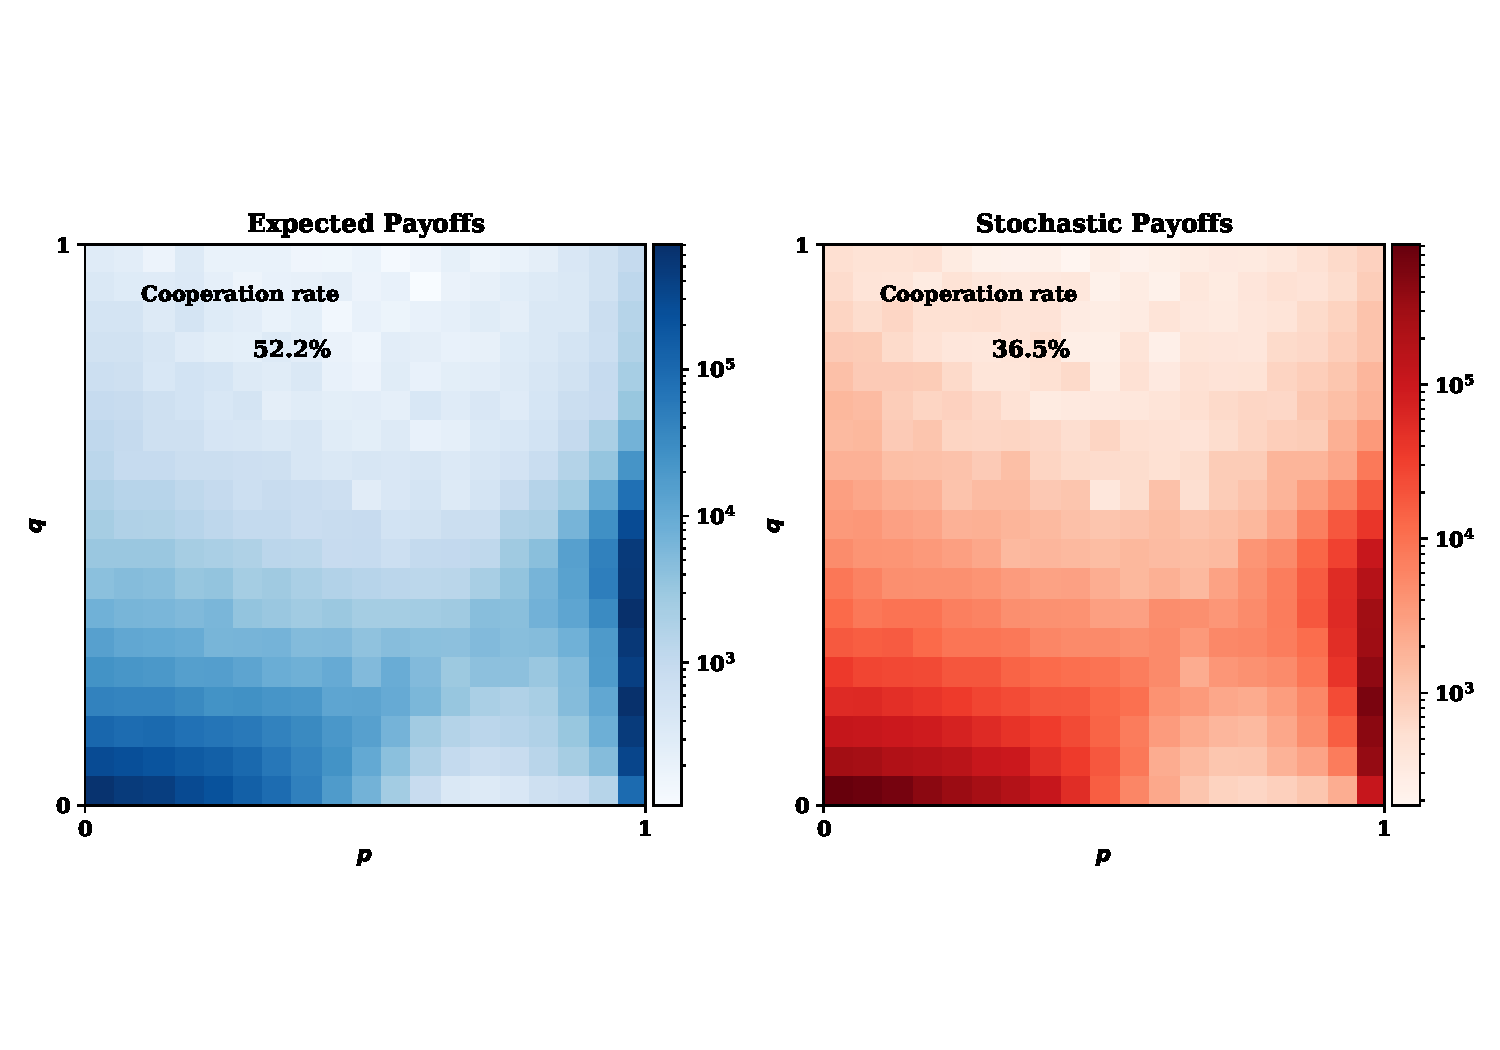
\includegraphics[width=\textwidth]{static/expected_and_stochastic_for_donation_game.pdf}
%     \caption{Blah blah.}
% \end{figure}



% \section{Pairwise imitation dynamics under stochastic payoff evaluation}

% \subsection{Basic setup} \label{Sec:BasicSetup}
% In the following we consider a population of size $N$, where $N$ is even. We assume mutations are sufficiently rare such that at any point in time at most two different strategies are present in the population. Suppose there are $N\!-\!k$ players who use the strategy $S_1\!=\!(y_1,p_1,q_1)$, whereas $k$ players use the strategy $S_2\!=\!(y_2,p_2,q_2)$. We refer to these two player types as `residents' and `mutants', respectively. 

% Each step of the evolutionary process consists of two stages, a game stage and an updating stage. In the game stage, each player is randomly matched with some other player in the population to interact in one instance of the repeated prisoner's dilemma. 
% In the updating stage, two players are randomly drawn from the population, a `learner' and a `role model'. Given that the learner's payoff in the last round is $u_L\!\in\! \mathcal{U}$ and that the role model's last round's payoff $u_M\!\in\! \mathcal{U}$, we assume the learner adopts the role model's strategy with probability 
% \begin{equation} \label{Eq:rho}
% \rho(u_L, u_M) = \frac{1}{1\!+\!\exp\big[ \!-\!\beta (u_M\!-\!u_L) \big]}. 
% \end{equation}
% The parameter $\beta\!\ge\!0$ corresponds to the strength of selection.

% We iterate this basic evolutionary step until either the mutant strategy goes extinct, or until it fixes in the population (in which case the mutant strategy becomes the new resident strategy). After either outcome, we introduce a new mutant strategy $S'_2\!=\!(y_2',p_2',q_2')$ (uniformly chosen from all reactive strategies at random), and we set the number of mutants to $k\!=\!1$. This process of mutation and fixation/extinction is then iterated many times. 

% We compare this process for stochastic payoff evaluation with the analogous process where players update their strategies with respect to their {\it expected} payoffs,
% \begin{equation} \label{Eq:ExpPay}
% \begin{array}{lcrcr}
% \displaystyle \pi_1	&=	&\displaystyle \frac{N\!-\!k\!-\!1}{N-1}\cdot \langle\mathbf{v}(S_1,S_1),\mathbf{u}\rangle	&+	&\displaystyle\frac{k}{N-1}\cdot \langle\mathbf{v}(S_1,S_2),\mathbf{u}\rangle,\\[0.5cm]
% \displaystyle \pi_2	&=	&\displaystyle\frac{N-k}{N-1}\cdot \langle\mathbf{v}(S_2,S_1),\mathbf{u}\rangle&+	&\displaystyle\frac{k-1}{N-1}\cdot \langle\mathbf{v}(S_2,S_2),\mathbf{u}\rangle.\\
% \end{array}
% \end{equation}
% In the limit of no discounting, $\delta\!\rightarrow\! 1$, this process based on expected payoffs has been considered in~\cite{imhof2010stochastic}. 

% \subsection{Fixation probabilities under stochastic payoff evaluation}
% Given that $N\!-\!k$ players use the resident strategy $S_1\!=\!(y_1,p_1,q_1)$ and that the remaining $k$ players use the mutant strategy $S_2\!=\!(y_2,p_2,q_2)$, the probability that the number of mutants increases by one in one step of the evolutionary process can be written as
% \begin{equation}
% \lambda^+_k=\frac{N\!-\!k}{N}\cdot \frac{k}{N}\cdot \sum_{u_1,u_2\in\mathcal{U}} x(u_1,u_2)\cdot \rho(u_1,u_2).
% \end{equation}
% In this expression, $(N\!-\!k)/N$ is the probability that the randomly chosen learner is a resident, and $k/N$ is the probability that the role model is a mutant. The sum corresponds to the total probability that the learner adopts the role model's strategy over all possible payoffs $u_1$ and $u_2$ that the two player may have received in their respective last rounds. We use $x(u_1,u_2)$ to denote the probability that the randomly chosen resident obtained a payoff of $u_1$ in the last round of his respective game, and that the mutant obtained a payoff of $u_2$. Given that the payoffs are $u_1$ and $u_2$, the imitation probability is then given by $\rho(u_1,u_2)$, as specified by Eq.~(\ref{Eq:rho}). The probability that the respective payoffs of the players are given by $u_1$ and $u_2$ can be calculated as
% \begin{equation}
% \setlength{\arraycolsep}{1pt}
% \begin{array}{llrl}
% x(u_1,u_2)	 &=&\displaystyle \frac{1}{N\!-\!1}\cdot  &v_{u_1}(S_1,S_2)\cdot 1_{(u_1,u_2)\in \mathcal{U}^2_F}\\[0.5cm]
% &+	
% &\displaystyle \left(1\!-\!\frac{1}{N\!-\!1}\right)  
% &\left[ \frac{k\!-\!1}{N\!-\!2}\frac{k\!-\!2}{N\!-\!3} v_{u_1}(S_1,S_2) v_{u_2}(S_2,S_2) + 
%  \frac{k\!-\!1}{N\!-\!2}\frac{N\!-\!k\!-\!1}{N\!-\!3} v_{u_1}(S_1,S_2) v_{u_2}(S_2,S_1)\right.\\[0.5cm]
% &&&\left. +\frac{N\!-\!k\!-\!1}{N\!-\!2}\frac{k\!-\!1}{N\!-\!3} v_{u_1}(S_1,S_1) v_{u_2}(S_2,S_2) + 
%  \frac{N\!-\!k\!-\!1}{N\!-\!2}\frac{N\!-\!k\!-\!2}{N\!-\!3} v_{u_1}(S_1,S_1) v_{u_2}(S_2,S_1)\right].
% \end{array}
% \end{equation}
% The first term on the right side corresponds to the case that the learner and the role model happened to be matched during the game stage, which happens with probability $1/(N\!-\!1)$. In that case, we note that only those payoff pairs can occur that are feasible in a direct interaction, $(u_1,u_2)\in \mathcal{U}^2_F:=\big\{ (R,R), (S,T), (T,S), (P,P) \big\}$, as represented by the respective indicator function. Otherwise, if the learner and the role model did not interact directly, we need to distinguish four different cases, depending on whether the learner was matched with a resident or a mutant, and depending on whether the role model was matched with a resident or a mutant. 

% Analogously, we can calculate the probability that the number of mutants decreases by one in one step of the evolutionary process. This probability is
% \begin{equation}
% \lambda^-_k=\frac{N\!-\!k}{N}\cdot\frac{k}{N} \sum_{u_1,u_2\in\mathcal{U}} x(u_1,u_2)\cdot \rho(u_2,u_1).
% \end{equation}
% The fixation probability of the mutant strategy then takes the standard form \cite{nowak2004emergence},
% \begin{equation}
% \varphi = \frac{1}{1+\sum_{i=1}^{N-1}\prod_k^i \frac{\lambda^-_k}{\lambda^+_k}}.
% \end{equation}


% \subsection{Invasion analysis of ALLD into GTFT}

% In the following, we apply the above formalism to calculate how easily a single ALLD mutant can invade into a resident population with strategy GTFT. In that case, $S_1=(1,1,q)$, $S_2\!=\!(0,0,0)$, and $k\!=\!1$. When two GTFT players interact in the game, their respective probabilities for each of the four outcomes in the last round simplify to
% \begin{equation}
% \begin{array}{cc}
% v_R(GTFT,GTFT)=1, &v_S(GTFT,GTFT)=0,\\
% v_T(GTFT,GTFT)=0, &v_P(GTFT,GTFT)=0.
% \end{array}
% \end{equation}
% On the other hand, if an ALLD player interacts with a GTFT player, the respective probabilities according to Eq.~(\ref{Eq:LastRound}) become
% \begin{equation}
% \begin{array}{ll}
% v_R(ALLD,GTFT)=0,	&v_S(ALLD,GTFT)=0,\\
% v_T(ALLD,GTFT)=1\!-\!\delta+\delta q,~~~ 	&v_P(ALLD,GTFT)=\delta(1\!-\!q).
% \end{array}
% \end{equation}
% As a consequence, we obtain the following probabilities $x(u_1,u_2)$ that the payoff of a randomly chosen GTFT player is $u_1$ and that the payoff of the ALLD player is $u_2$,
% \begin{equation}
% \begin{array}{l}
% \displaystyle x(R,T)=\frac{N-2}{N-1} \cdot (1\!-\!\delta\!+\!\delta q),\\[0.5cm]
% \displaystyle x(R,P)=\frac{N-2}{N-1} \cdot \delta(1\!-\!q),\\[0.5cm]
% \displaystyle x(S,T)=\frac{1}{N-1} \cdot (1\!-\!\delta\!+\!\delta q), \\[0.5cm]
% \displaystyle x(P,P)=\frac{1}{N-1} \cdot \delta(1\!-\!q). \\[0.5cm]
% \displaystyle x(u_1,u_2)=0	~~~\text{for all other payoff pairs}~(u_1,u_2).
% \end{array}
% \end{equation}
% As a consequence, we can calculate the ratio of transition probabilities as 
% \begin{equation}
% \frac{\lambda_1^+}{\lambda_1^-}=\displaystyle \frac{\displaystyle \frac{N-2}{N-1} \cdot \left(\frac{1\!-\!\delta\!+\!\delta q}{1\!+\!\exp[-\beta(T\!-\!R)]}
% \!+\! \frac{\delta(1-q)}{1\!+\!\exp[-\beta(P\!-\!R)]}\right)
% + \frac{1}{N\!-\!1} \left(\frac{1-\delta+\delta q}{1+\exp[-\beta (T\!-\!S)]}
% \!+\! \frac{\delta(1-q)}{2}\right)}
% {\displaystyle \frac{N-2}{N-1} \cdot \left(\frac{1\!-\!\delta\!+\!\delta q}{1\!+\!\exp[-\beta(R\!-\!T)]}
% \!+\! \frac{\delta(1-q)}{1\!+\!\exp[-\beta(R\!-\!P)]}\right)
% + \frac{1}{N\!-\!1} \left(\frac{1-\delta+\delta q}{1+\exp[-\beta (S\!-\!T)]}
% \!+\! \frac{\delta(1-q)}{2}\right)}.
% \end{equation}

% \noindent
% In particular, in the limit of strong selection $\beta \rightarrow \infty$ and large populations $N\!\rightarrow \infty$, we obtain
% \begin{equation}
% \frac{\lambda_1^+}{\lambda_1^-}=
% \frac{ 1\!-\!\delta+\delta q}{\delta (1-q)}.
% \end{equation}
% This ratio is smaller than 1 (such that ALLD is disfavored to invade) if $q<1\!-\!1/(2\delta)$. For infinitely repeated games, $\delta\!\rightarrow\!1$, this condition becomes $q\!<\!1/2$ (for $q\!=\!1/2$, the payoff of the ALLD player is $T\!>\!R$ for half of the time, and it is $P\!<\!R$ for the other half. The probability that the number of mutants increase by one equals the probability that the mutant goes extinct). 


% % \subsection{Simulation results}

% % \FigEvoProc -- \FigResultsOverPara~show simulation results for the above described process. \FigEvoProc~depicts the evolving conditional cooperation probabilities $p$ and $q$ (assuming that the discount factor~$\delta$ and the benefit $b$ are comparably high). The left panel corresponds to the standard scenario considered in the previous literature. It considers players who use expected payoffs (\ref{Eq:ExpPay}) to update their strategies. The right panel shows the scenario considered herein, in which players update their strategies based on their last round's payoff. The figure suggests that when updating is based on expected payoffs, players tend to be more generous (their $q$-values are higher on average). In addition, players are generally more cooperative. 

% % \begin{figure}[t!]
% % \centering
% % 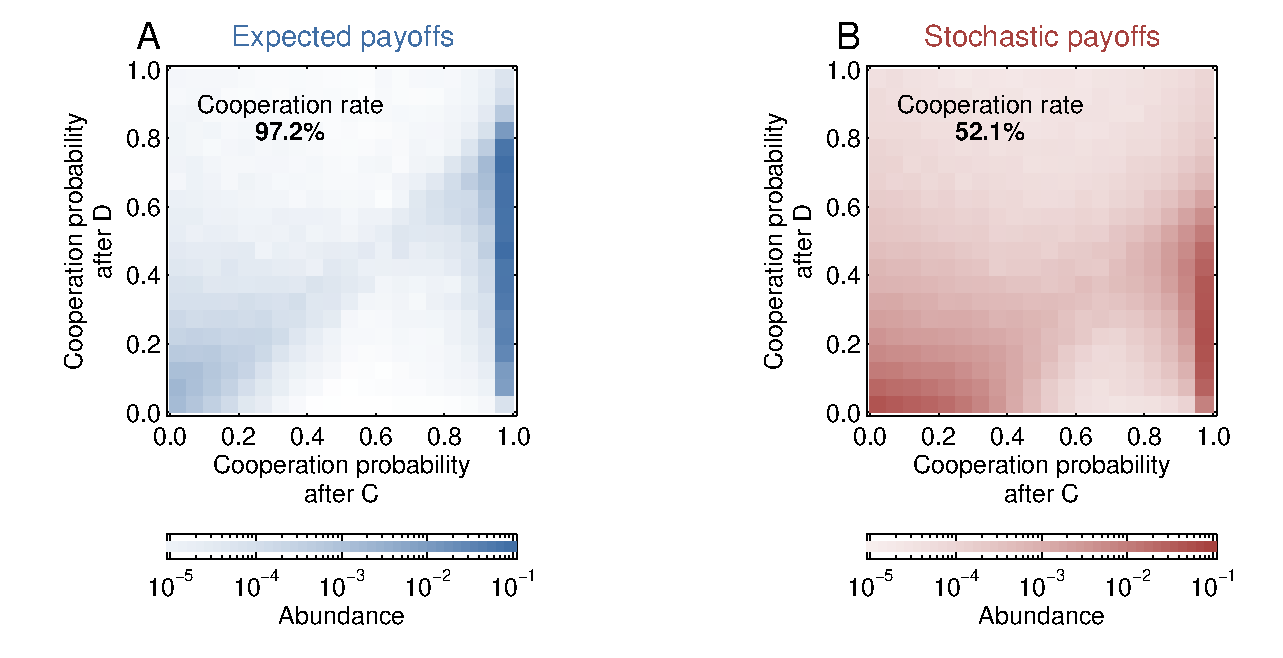
\includegraphics[width=0.75\textwidth]{Fig1} 
% % \caption{{\bf Evolutionary dynamics under expected payoffs (left) and stochastic payoffs (right).} 
% % We have run two simulations of the evolutionary process described in Section~\ref{Sec:BasicSetup} for $T\!=\!10^7$ time steps. For each time step, we have recorded the current resident population ($y,p,q$). Since simulations are run for a relatively high continuation probability of $\delta\!=\!0.999$, we do not report the players' initial cooperation probability $y$. The graphs show how often the resident population chooses each combination ($p,q$) of conditional cooperation probabilities in the subsequent rounds. ({\bf A}) If players update based on their expected payoffs, the resident population typically applies a strategy for which $p\!\approx\!1$ and $q\!\le\!1\!-\!c/b\!=\!0.9$. The cooperation rate within the resident population (averaged over all games and over all time steps) is close to 100\%. ({\bf B}) When players update their strategies based on their realized payoffs in the last round, there are two different predominant behaviors. The resident population either consists of defectors (with $p\!\approx\!q\!\approx\!0$) or of conditional cooperators. In the latter case, the maximum level of $q$ consistent with stable cooperation is somewhat smaller compared to the expected-payoff setting, $q\!<\!0.5$. Also the resulting cooperation rate is smaller. On average, players cooperate roughly in half of all rounds. Parameters: $N\!=\!100$, $b\!=\!3$, $c\!=\!1$, $\beta\!=\!1$, $\delta\!=\!0.999$.}
% % \end{figure}

% % To obtain some intuition for this result, we have recorded which mutant strategies typically invade into an ALLD population, and which mutants invade into a GTFT population, for each of the two scenarios (\FigInvAnalysis). Compared to expected-payoff updating, the stochastic scenario drastically reduces the stability of GTFT. On average, it takes fewer mutants until a GTFT population is successfully invaded. Moreover, successful mutants  tend to be less cooperative. 

% % \begin{figure}[t!]
% % \centering
% % 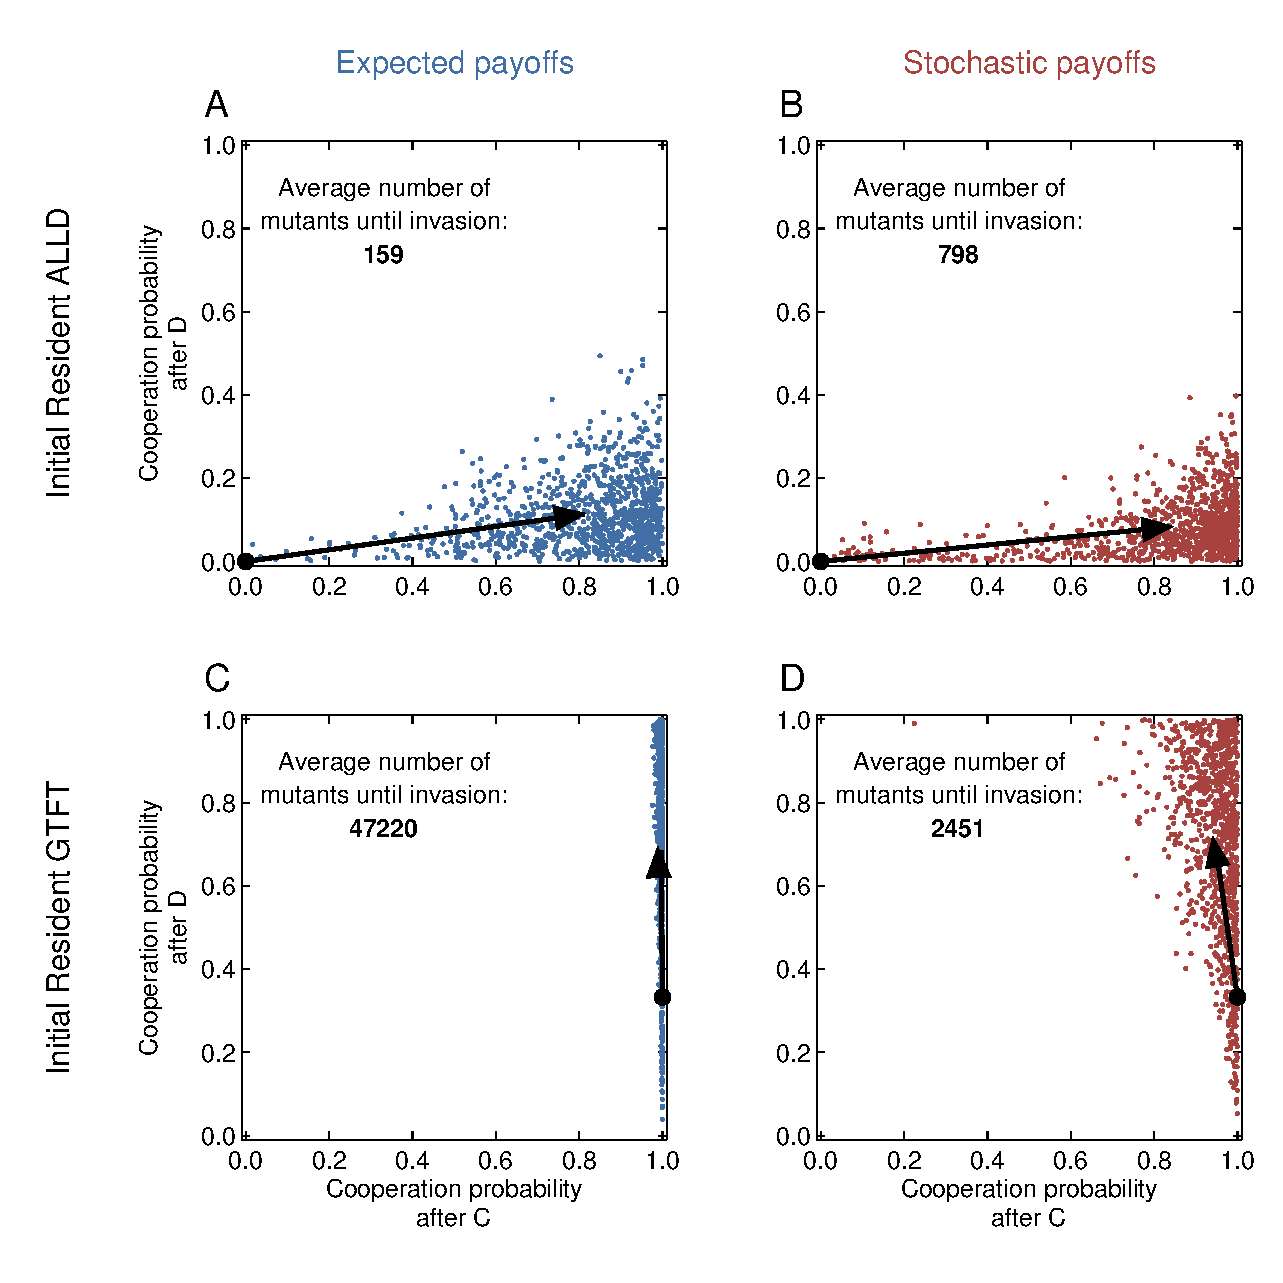
\includegraphics[width=0.75\textwidth]{Fig2} ~\\[-0.6cm]
% % \caption{{\bf Invasion into ALLD and into GTFT for the two evolutionary scenarios.} 
% % For this figure, we either consider a resident population of ALLD players (top) or of GTFT players (bottom). In each case, we have run 1,000 independent simulations of the evolutionary process described in Section~\ref{Sec:BasicSetup}. The colored dots within the four panels depict which mutant strategies successfully invaded into the respective resident population. The black arrow indicates the average over all successful mutant strategies. In addition, we have recorded how many mutant strategies need to be introduced into the population until the resident becomes replaced. Stochastic payoffs tend to increase the time until ALLD is invaded, and they reduce the time until GTFT is invaded. Parameters are the same as in \FigEvoProc. Strategies are defined as $ALLD\!=\!(0,0,0)$ and $GTFT=(1,1,1/3)$.}
% % ~\\[0.4cm]
% % 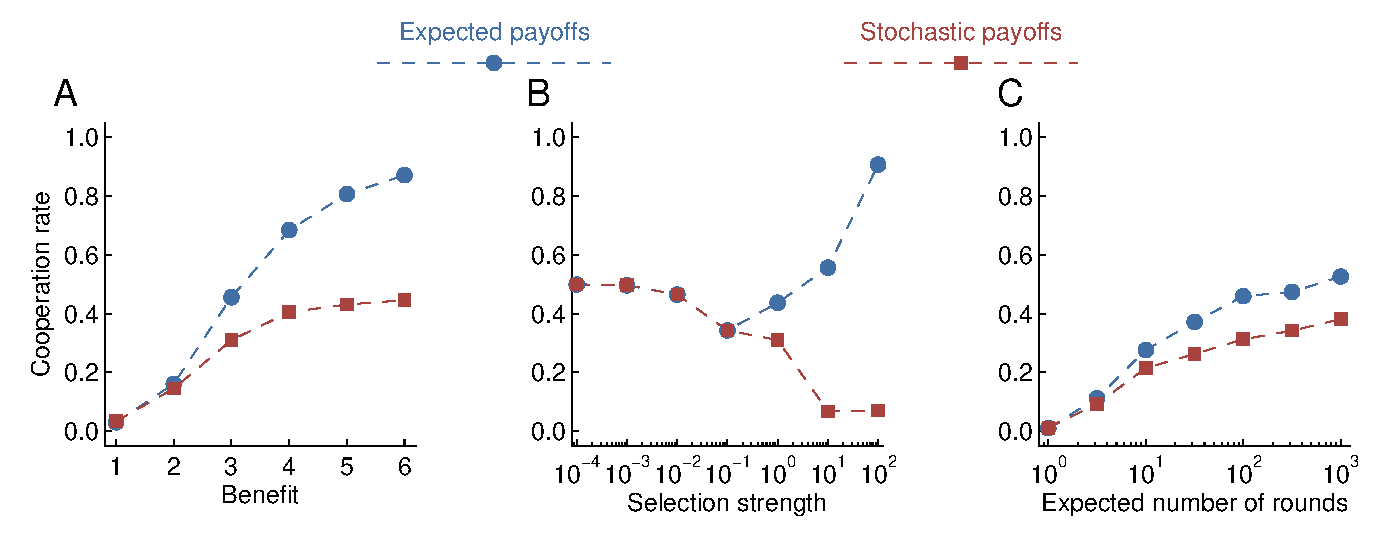
\includegraphics[width=0.8\textwidth]{Fig3} 
% % \caption{{\bf The evolution of cooperation for different parameter values.} 
% % While the previous figures depict the evolutionary outcome for fixed parameter values, here we vary the benefit of cooperation $b$, the strength of selection $\beta$, and the expected number of rounds, $1/(1\!-\!\delta)$. In all cases, stochastic payoff evaluation tends to reduce the evolving cooperation rates. Unless explicitly varied, the parameters of the simulation are $N\!=\!100$, $b\!=\!3$, $c\!=\!1$, $\beta\!=\!1$, $\delta\!=\!0.99$. Simulations are run for $T\!=\!5\times 10^6$ time steps for each parameter combination.}
% % \end{figure}

% % Finally, we have also explored how the evolving cooperation rates change as we vary the benefit $b$, the selection strength $\beta$, and the discount factor $\delta$ (\FigResultsOverPara). In all three cases, we find that the two scenarios yield similar cooperation rates when the respective parameters are small. Once there is a high benefit to cooperation, strong selection, or a high expected number of rounds, updating based on expected payoffs yields higher cooperation rates.

\clearpage
\newpage


\bibliographystyle{unsrt}
\bibliography{bibliography.bib}



\end{document}
